% -----------------------------------------------------------------------------
%       Centro Federal de Educação Tecnológica de Minas Gerais - CEFET-MG
%
%   Modelo de trabalho acadêmico em conformidade com as normas da ABNT
%   (Tese de Doutorado, Dissertação de Mestrado ou Projeto de Qualificação)
%
%    Projeto hospedado em: https://github.com/cfgnunes/latex-cefetmg
%
%    Autores: Cristiano Nunes <cfgnunes@gmail.com>
%             Henrique Borges <henrique@cefetmg.br>
% -----------------------------------------------------------------------------

\documentclass[%
    %twoside,              % Impressão em frente (anverso) e verso
    oneside,               % Impressão apenas no anverso
]{cefetmg}

\usepackage[%
    alf,
    abnt-emphasize=bf,
    bibjustif,
    recuo=0cm,
    abnt-doi=expand,       % Expande endereço iniciado com doi: para http://dx.doi.org/
    abnt-url-package=url,  % Utiliza o pacote url
    abnt-refinfo=yes,      % Utiliza o estilo bibliográfico abnt-refinfo
    abnt-etal-cite=3,
    abnt-etal-list=3,
    abnt-thesis-year=final
]{abntex2cite}             % Configura as citações bibliográficas

% -----------------------------------------------------------------------------
% Pacotes utilizados
% -----------------------------------------------------------------------------
\usepackage[utf8]{inputenc}                      % Codificação do documento
\usepackage[T1]{fontenc}                         % Seleção de código de fonte
\usepackage{booktabs}                            % Réguas horizontais em tabelas
\usepackage{color, colortbl}                     % Controle de cores
\usepackage{float}                               % Tabelas/figuras em ambiente multicolunas
\usepackage{graphicx}                            % Inclusão de gráficos
\usepackage{icomma}                              % Uso de vírgulas em expressões matemáticas
\usepackage{indentfirst}                         % Recua o primeiro parágrafo de cada seção
\usepackage{microtype}                           % Melhora a justificação do documento
\usepackage{multirow, array}                     % Tabelas com múltiplas linhas e colunas
\usepackage{subeqnarray}                         % Subenumeração de equações
\usepackage{verbatim}                            % Apresentar texto tal como escrito no documento
\usepackage{amsfonts, amssymb, amsmath}          % Fontes e símbolos matemáticos
\usepackage[algoruled, portuguese]{algorithm2e}  % Algoritmos em português
\usepackage[scaled]{helvet}                      % Usa a fonte Helvetica
%\usepackage{times}                              % Usa a fonte Times
%\usepackage{palatino}                           % Usa a fonte Palatino
%\usepackage{lmodern}                            % Usa a fonte Latin Modern
%\usepackage[bottom]{footmisc}                   % Notas de rodapé sempre na mesma posição
%\usepackage{ae, aecompl}                        % Fontes de alta qualidade
%\usepackage{latexsym}                           % Símbolos matemáticos
%\usepackage{lscape}                             % Páginas em modo paisagem
%\usepackage{picinpar}                           % Dispor imagens em parágrafos
%\usepackage{scalefnt}                           % Redimensionar tamanho da fonte
%\usepackage{subfig}                             % Posicionamento de figuras
%\usepackage{upgreek}                            % Fonte letras gregas

% Redefine a fonte para uma fonte similar a Arial (fonte Helvetica)
\renewcommand*\familydefault{\sfdefault}

% -----------------------------------------------------------------------------
% Configurações de aparência do PDF final
% -----------------------------------------------------------------------------
\makeatletter
\hypersetup{%
    portuguese,
    colorlinks=true, % true: links coloridos; false: links em caixas de texto
    linkcolor=blue,  % Cor dos links internos
    citecolor=blue,  % Cor dos links para as referências bibliográficas
    filecolor=blue,  % Cor dos links para arquivos
    urlcolor=blue,   % Cor dos links de URLs
    breaklinks=true,
    pdftitle={\@title},
    pdfauthor={\@author},
    pdfkeywords={abnt, latex, abntex, abntex2}
}
\makeatother

% Altera o aspecto da cor azul
\definecolor{blue}{RGB}{41,5,195}

% Redefinição de labels
\renewcommand{\algorithmautorefname}{Algoritmo}
\def\equationautorefname~#1\null{Equa\c c\~ao~(#1)\null}

% Cria o índice remissivo
\makeindex

% Hifenização de palavras que não estão no dicionário
\hyphenation{%
    qua-dros-cha-ve
    Kat-sa-gge-los
}

% -----------------------------------------------------------------------------
% Inclui os arquivos do trabalho acadêmico
% -----------------------------------------------------------------------------

% Insere e constrói alguns elementos pré-textuais para gerar capa,
% folha de rosto e folha de aprovação
% -----------------------------------------------------------------------------
% Capa
% -----------------------------------------------------------------------------

% -----------------------------------------------------------------------------
% ATENÇÃO:
% Caso algum campo não se aplique ao seu documento - por exemplo, em seu
% trabalho não houve coorientador - não comente o campo, apenas deixe vazio,
% assim: \campo{}
% -----------------------------------------------------------------------------

% -----------------------------------------------------------------------------
% Dados do trabalho acadêmico
% -----------------------------------------------------------------------------

\titulo{Desenvolvimento de produtos utilizando Design System como ponte entre Designers e Desenvolvedores}
\autor{Luís Cláudio Assis do Nascimento}
\local{Belo Horizonte}
\data{Junho de 2019} % Normalmente se usa apenas mês e ano

% -----------------------------------------------------------------------------
% Natureza do trabalho acadêmico
% Use apenas uma das opções: Tese (p/ Doutorado), Dissertação (p/ Mestrado) ou
% Projeto de Qualificação (p/ Mestrado ou Doutorado), Trabalho de Conclusão de
% Curso (Graduação)
% -----------------------------------------------------------------------------

\projeto{Trabalho de Conclusão de Curso}

% -----------------------------------------------------------------------------
% Título acadêmico
% Use apenas uma das opções:
% - Se a natureza for Tese, coloque Doutor
% - Se a natureza for Dissertação, coloque Mestre
% - Se a natureza for Projeto de Qualificação, coloque Mestre ou Doutor
% - Se a natureza for Trabalho de Conclusão de Curso, coloque Bacharel
% -----------------------------------------------------------------------------

\tituloAcademico{Bacharel}

% -----------------------------------------------------------------------------
% Área de concentração e linha de pesquisa
% Observação: Indique o nome da área de concentração e da linha de pesquisa do
% programa de Pós-graduação nas quais este trabalho se insere. Se a natureza
% for Trabalho de Conclusão de Curso, deixe ambos os campos vazios.
% -----------------------------------------------------------------------------

\areaconcentracao{Engenharia de Software e Interação Humano-Computador}
% \linhapesquisa{Arquitetura e Design de Sistemas}

% -----------------------------------------------------------------------------
% Dados da instituição
% Observação: A logomarca da instituição deve ser colocada na mesma pasta que
% foi colocada o documento principal com o nome de "logoInstituicao".
% O formato pode ser: pdf, jpf, eps. Se a natureza for Trabalho de Conclusão
% de Curso, coloque em "programa' o nome do curso de graduação.
% -----------------------------------------------------------------------------

\instituicao{Centro Federal de Educação Tecnológica de Minas Gerais}
\programa{Curso de Engenharia de Computação}
%\programa{Curso de Engenharia de Computação}
\logoinstituicao{0.2}{./04-figuras/logo-instituicao.pdf}

% -----------------------------------------------------------------------------
% Dados do(s) orientador(es)
% -----------------------------------------------------------------------------

\orientador{Cristiano Amaral Maffort}
%\orientador[Orientadora:]{Nome da orientadora}
\instOrientador{Centro Federal de Educação Tecnologica de Minas Gerais}

% \coorientador{Nome do coorientador}
%\coorientador[Coorientadora:]{Nome da coorientadora}
% \instCoorientador{Instituição do coorientador}

% -----------------------------------------------------------------------------
% Folha de Rosto
% -----------------------------------------------------------------------------

% Trabalho de Conclusão de Curso
\preambulo{{\imprimirprojeto} apresentado ao Curso de Engenharia de Computação do Centro Federal de Educação Tecnológica de Minas Gerais, como requisito parcial para a obtenção do título de {\imprimirtituloAcademico} em Engenharia de Computação.}

% Projeto de qualificação de Mestrado ou Doutorado
% \preambulo{{\imprimirprojeto} apresentado ao Programa de \mbox{Pós-graduação} em Modelagem Matemática e Computacional do Centro Federal de Educação Tecnológica de Minas Gerais, como requisito parcial para a obtenção do título de {\imprimirtituloAcademico} em Modelagem Matemática e Computacional.}

% Dissertação de Mestrado
%\preambulo{{\imprimirprojeto} apresentada ao Programa de \mbox{Pós-graduação} em Modelagem Matemática e Computacional do Centro Federal de Educação Tecnológica de Minas Gerais, como requisito parcial para a obtenção do título de {\imprimirtituloAcademico} em Modelagem Matemática e Computacional.}

% Tese de Doutorado
%\preambulo{{\imprimirprojeto} apresentada ao Programa de \mbox{Pós-graduação} em Modelagem Matemática e Computacional do Centro Federal de Educação Tecnológica de Minas Gerais, como requisito parcial para a obtenção do título de {\imprimirtituloAcademico} em Modelagem Matemática e Computacional.}

% -----------------------------------------------------------------------------
% Edite este arquivo comentando as linhas que não se aplicam ao tipo de
% documento acadêmico pretendido.
% -----------------------------------------------------------------------------

% -----------------------------------------------------------------------------
% Folha de Aprovação
% -----------------------------------------------------------------------------

\textopadraofolhadeaprovacao{}

\avaliacaotrab{Avaliação do Trabalho de Conclusão de Curso}

\corpoavaliacao{
Aluno: Luís Cláudio Assis do Nascimento \\
Título do trabalho: Desenvolvimento de produtos utilizando Design System como ponte entre Designers e Desenvolvedores \\
Data da defesa: 18/06/2019 \\
Horário: 13:30 \\
Local da defesa: CEFET-MG Campus II, Avenida Amazonas 7675. Prédio 17 (DECOM), sala 401
}

\initprof{O presente Trabalho de Conclusão de Curso foi avaliado pela seguinte banca:}

\orientadoravaliacao{
Cristiano Amaral Maffort - Orientador \\ 
Departamento de Computação \\
Centro Federal de Educação Tecnológica de Minas Gerais
}

\profavaliacaoum{
Flávio Roberto dos Santos Coutinho - Membro da banca de avaliação \\ 
Departamento de Computação \\
Centro Federal de Educação Tecnológica de Minas Gerais
}

\profavaliacaodois{
Glívia Angélica Rodrigues Barbosa - Membro da banca de avaliação \\ 
Departamento de Computação \\
Centro Federal de Educação Tecnológica de Minas Gerais
}

\begin{document}

% Insere os elementos pré-textuais
\pretextual
\imprimircapa                                            % Inclui Capa
\imprimirfolhaderosto{}                                  % Inclui Folha de rosto
\imprimirfolhadeaprovacao{}                              % Inclui Folha de aprovação
% -----------------------------------------------------------------------------
% Agradecimentos
% -----------------------------------------------------------------------------

\begin{agradecimentos}

Família em primeiro lugar. Obrigado mãe, pai e irmã. Sem seu apoio e carinho eu nada seria. Vocês são meu estimulo a seguir em frente, superando com coragem, ética e garra todos os desafios que surgem a minha frente.

Agradeço a minha namorada, Gabriella, que me apoia e acredita no meu potencial. Seu amor e carinho, que me surpreendem todos os dias, me motivam a ser uma pessoa melhor. Você é muito importante pra mim e é peça fundamental dessa conquista.

A todos os amigos que acumulei ao longo da vida. Meu convívio com vocês moldou a pessoa que sou hoje. Saber que posso contar com vocês a qualquer momento é algo muito importante para mim.

Agradeço a Dito, por me dar a oportunidade de compartilhar um pouco do trabalho incrível que realizamos juntos todos os dias. Trabalhar em uma empresa de tamanho calíbre, com pessoas tão excelentes em tudo o que fazem, é um privilégio para poucos.

Agradeço ao CEFET-MG e a todo o corpo docente e discente dessa organização. Devo muito do que conquistei profissionalmente à excelência do trabalho de vocês.

A todas essas fontes de inspiração, o meu mais sincero obrigado.

\end{agradecimentos}
     % Agradecimentos
% -----------------------------------------------------------------------------
% Resumo
% -----------------------------------------------------------------------------

\begin{resumo}
    Reusabilidade e consistência de interfaces de usuário, tanto em termos de design quanto a nível de implementação, vem apresentando problemas desde a popularização das interfaces gráficas de usuário. Bibliotecas de componentes se propuseram a resolver tais problemas, entretanto, devido à vigente segregação entre os domínios do designer e do desenvolvedor, por muito tempo seu objetivo final não foi alcançado. Recentemente um novo conceito chamado \textit{design system} foi proposto como abordagem para a resolução destes problemas. Pretendo avaliar a eficácia e viabilidade do novo paradigma, este trabalho se dedica a realizar um experimento prático em uma empresa de tecnologia de médio porte. O experimento foi dividido em cinco momentos. O primeiro deles destinado à revisão da literatura e de trabalhos relacionado, tanto no âmbito acadêmico quanto no industrial. Em seguida, foram realizadas entrevistas com designers e desenvolvedores \textit{frontend} da empresa avaliada, com o objetivo de comprovar a necessidade de implementação de um \textit{design system}. Seguiu-se com a construção de uma biblioteca de componentes, em um formato de protótipo. O quarto estágio foi destinado à criação de páginas Web embasadas no protótipo de biblioteca de componentes construído anteriormente. Finaliza-se com o detalhamento da avaliação de resultados. De maneira geral, o experimento realizado contribuiu com a ideia de que um \textit{design system} deve ser solução para problemas de escalabilidade e comunicação de um produto.

    \textbf{Palavras-chave}: \textit{Design System}. \textit{Atomic Design}.
\end{resumo}

% -----------------------------------------------------------------------------
% Escolha de 3 a 6 palavras ou termos que descrevam bem o seu trabalho.
% As palavras-chaves são utilizadas para indexação. A letra inicial de cada
% palavra deve estar em maiúsculas. As palavras-chave são separadas por ponto.
% -----------------------------------------------------------------------------
          % Resumo na língua vernácula
% -----------------------------------------------------------------------------
% Lista de Figuras
% -----------------------------------------------------------------------------

\pdfbookmark[0]{\listfigurename}{lof}
\listoffigures*
\cleardoublepage

% -----------------------------------------------------------------------------
% Não é necessário editar este arquivo. A lista é gerada automaticamente.
% -----------------------------------------------------------------------------
      % Lista de figuras
% -----------------------------------------------------------------------------
% Lista de Tabelas
% -----------------------------------------------------------------------------

\pdfbookmark[0]{\listtablename}{lot}
\listoftables*
\cleardoublepage

% -----------------------------------------------------------------------------
% Não é necessário editar este arquivo. A lista é gerada automaticamente.
% -----------------------------------------------------------------------------
      % Lista de tabelas
% -----------------------------------------------------------------------------
% Lista de Quadros
% -----------------------------------------------------------------------------

\pdfbookmark[0]{\listofquadrosname}{loq}
\listofquadros*
\cleardoublepage

% -----------------------------------------------------------------------------
% Não é necessário editar este arquivo. A lista é gerada automaticamente.
% -----------------------------------------------------------------------------
      % Lista de quadros
% -----------------------------------------------------------------------------
% Lista de Siglas
% -----------------------------------------------------------------------------

\begin{siglas}
    \item[LED] \textit{Light emmiter diode}, ou diodo emissor de luz
    \item[GUI] \textit{Grafical User Interface}, ou interface de usuário gráfica
    \item[UX] \textit{User Experience}, ou experiência do usuário
    \item[HTML] \textit{Hypertext Markup Language}, ou Linguagem de marcação de Hipertexto
    \item[NPS] \textit{Net Promoter Score} 
\end{siglas}

% -----------------------------------------------------------------------------
% Edite a lista acima para definir as siglas utilizadas neste trabalho.
% -----------------------------------------------------------------------------
       % Lista de siglas
% -----------------------------------------------------------------------------
% Sumário
% -----------------------------------------------------------------------------

\pdfbookmark[0]{\contentsname}{toc}
\tableofcontents*
\cleardoublepage

% -----------------------------------------------------------------------------
% Não é necessário editar este arquivo. O sumário é gerado automaticamente.
% -----------------------------------------------------------------------------
            % Sumário

% Insere os elementos textuais
\textual
% -----------------------------------------------------------------------------
% Introdução
% -----------------------------------------------------------------------------

\chapter{Introdução}
\label{chap:introducao}

O valor do design de produto só começou a ser reconhecido recentemente perante a indústria de software moderna. Na virada do último milênio, a experiência do usuário (UX) era simplismente negligenciada, não sendo tratada como uma prioridade de negócio para a maioria das empresas de tecnologia. Entretanto, conforme as tecnologias foram amadurecendo e a competição entre empresas de desenvolvimento de software se tornaram mais acirradas, o design e a experiência do usuário começaram a conquistar o seu espaço \cite{ruissalo2018operating}.

Ao mesmo tempo, escalar efetivamente os processos de design e desenvolvimento de software em grandes empresas não é tarefa simples. Conforme uma organização expande seu negócios, incrementando a quantidade de produtos e serviços oferecidos por meio do aumento do número de funcionários, novas problemas tendem a se manifestar. O gerenciamento do conhecimento compartilhado entre os diferentes times de uma organização é um problema comumente enfrentado por grandes empresas de desenvolvimento de software que adotam metodologias de desenvolvimento ágil. Problemas como reusabilidade de soluções e consistência em experiência do usuário logo começam a se manifestar \cite{ruissalo2018operating}.

Com o intuito de remediar problemas de reuso e consistência em interfaces de usuário, surgiram bibliotecas de componentes no universo de desenvolvimento e guias de estilo no universo do design \cite{ruissalo2018operating}. Entretanto, pela maneira como era construídos, tais artefatos não alcançavam seu propósito no longo termo, pois não havia conexão alguma entre ambos \cite{ruissalo2018operating}.

Recentemente, como meio de aproximação entre os contextos de desenvolvimento e design, um novo conceito emergiu da indústria: \textit{design system} \cite{kholmatova2017design}.

\section{Justificativa}
\label{sec:justificativa}

O termo \textit{time to marketing}, cada dia mais frequente no vocabulário de profissionais de produtos de tecnologia, reflete bem a realidade de um mercado acelerado e competitivo que é presenciado atualmente. Representa o intervalo de tempo entre a ideação e o lançamento de um produto, e espera-se que seja o quão curto possível. Fato é que, tal expectativa muitas vezes é frustrada por conta de uma arquitetura degradada, pouco escalável e pouco reusável dos sistemas.

Além disso, estudos comprovam que a maior parcela dos custos envolvidos em um sistema de software está concentrado em atividades de manutenção do produto \cite{softwareCost}. Em uma realidade de mercado onde os profissionais especializados em desenvolvimento de software estão cada dia mais valorizados, manter um sistema de difícil manutenção é bastante custoso.

\section{Motivação}
\label{sec:motivacao}

Como colaborador ativo de uma promissora empresa de tecnologia, o autor deste trabalho identificou na plataforma que manuseia diariamente, problemas arquiteturais que criam barreiras para a evolução do produto e, consequentemente, crescimento da organização. Ciente de que medidas deveriam ser tomadas imediatamente para reverter o atual cenário, foi realizado o presente trabalho afim de se encontrar alguma alternativa para os empencilhos identificados.

\section{Objetivos}
\label{sec:objetivos}

\subsection{Objetivo Geral}

O objetivo principal deste trabalho é comprovar a hipótese de que a implementação de um \textit{design system} em uma empresa de médio porte, é uma solução viável para problemas de escalabilidade de um produto estruturado por uma arquitetura degradada. Espera-se que ao final do projeto, o valor do \textit{design system} como ferramenta de centralização de conhecimento e padronização de artefatos de desenvolvimento seja reconhecido pela empresa em questão e que trabalhos sejam iniciados em direção ao seu desenvolvimento.

\subsection{Objetivos Específicos}

\begin{enumerate}
    \item Entrevistar designers e desenvolvedores \textit{frontend} da empresa, afim de entender as principais dores e frustrações por eles percebidas ao executar suas atividades diárias.
    \item Validar se os problemas identificados pelos os entrevistados são resolvidos por meio da implamentação de um \textit{design system}, de acordo com a literatura.
    \item Implementar o protótipo de uma biblioteca de componentes simples que consiga evidenciar as principais vantagens de se contruir interfaces de usuários baseadas em componentes desenvolvidos previamente.
\end{enumerate}{}

\section{Organização do trabalho}
\label{sec:organizacaoTrabalho}

Este trabalho foi organizado em 9 grandes capítulos, sendo a introdução o primeiro deles. No segundo capítulo serão discutidos alguns dos fundamentos teórico-conceituais mais importantes para a contextualização do leitor ao problema abordado. Logo em seguida, no capítulo 3, serão apresentados alguns dos trabalhos relacionados ao tema deste projeto, que foram divulgados na literatura e na indústria, e formam a principal referência para a sua construção. No capítulo 4 é apresentada a metodologia utilizada para o desenvolvimento do trabalho. Os capítulos 5, 6 e 7 são destinados a entrevistas com \textit{stakeholders}, desenvolvimento do protótipo de biblioteca de componentes e desenvolvimento de páginas web embasadas nesta biblioteca, respectivamente. A avaliação dos resultados obtidos ao longo do desenvolvimento do trabalho é discutida no capítulo 8, seguida das conclusões no Capítulo 9.

             % Introdução
% -----------------------------------------------------------------------------
% Fundamentação Teórica
% -----------------------------------------------------------------------------

\chapter{Fundamentação Teórica}
\label{chap:fundamentacaoTeorica}

O presente capítulo tem como objetivo discutir a teoria por trás do \textit{design system}. O capítulo é introduzido conceituando a idéia de \textit{design} de interação, apresentando o contexto do seu surgimento e os desafios que ele traz consigo. Logo em seguida, é discutida a questão da experiência do usuário no mercado de software moderno. Finaliza-se o capítulo, dissecando o \textit{design system} e por fim apresentando o \textit{atomic design} como proposta de metodologia para sua implementação.

\section{Design de Interação}
\label{sec:designInteracao}

Nos primórdios da era da computação, os primeiros sistemas computacionais eram criados para atender demandas dos próprios engenheiros que os criavam, ou eram destinados à usuários com um background técnico muito avançado. As interfaces com os computadores da época eram, em geral, baseadas em painéis com chaves e componentes que indicavam o estado atual dos circuitos internos do sistema (LEDs). Restava ao usuário final apenas uma extensa documentação a ser lida, de forma a de fato entender o comportamento do sistema \cite{preece2005design}.

Foi no final dos anos 70 e início dos anos 80, com o advento dos monitores e estações de trabalhos pessoais, que o design de interface passou a existir \cite{grudin1990computer}. Um dos principais desafios da época foi o desenvolvimento de sistemas acessíveis à pessoas comuns, de forma a auxiliá-las a desenvolver tarefas intelectuais simples, como escrever documentos por exemplo \cite{preece2005design}.

Para tornar isso possível, reuniram-se profissionais de diferentes áreas para estudar as novas possibilidades que o design de interface de usuários trazia consigo. Cientistas da computação, psicólogos, designers gráficos e designers de produtos uniram seus esforços para o estudo e desenvolvimento de interfaces gráficas (abreviadas GUI), de forma a atender à demanda latente por esse tipo de sistema. Nessa época muitos estudos foram feitos na área de design de produtos, com o intuito de entender a melhor maneira de estruturar os diferentes componentes visuais do sistema na interface de usuário \cite{preece2005design}.

Atualmente, segundo \cite{preece2005design}, entende-se como design de interação:
“Design de produtos interativos que fornecem suporte às atividades cotidianas das pessoas, seja no lar ou no trabalho. Significa criar experiências que melhoram e estendem a maneira como as pessoas trabalham, se comunicam e interagem”. 
O autor ainda faz uma breve analogia, embasado em Terry Winograd, ao descrever o design de interação. A analogia tem como base o questionamento das diferenças de pensamento entre arquitetos e engenheiros ao se depararem com o mesmo problema de se construir uma casa. O autor pondera que, o trabalho do arquiteto muito se assemelha à de um designer, com um caráter artístico, mais voltado para a usabilidade. Por outro lado, o engenheiro é associado ao desenvolvedor de software, com características bastante técnicas. Apesar de ser um um ponto de vista válido, o objetivo do presente trabalho é justamente questionar esse modelo de visão segregatória do mercado, onde os papéis de designers e desenvolvedores estão muitas vezes isolados. Deve-se haver uma linguagem comum entre designers e desenvolvedores, que proporcione uma rica troca de idéias entre os diferentes tipos de profissionais e garanta os benefícios de se ter times realmente multidisciplinares. A linguagem proposta para esse problema é o que se entende como \textit{Design System}.

\section{Experiência do usuário e o mercado de desenvolvimento de software moderno}
\label{experienciaUsuarioMercado}

O design de interação com foco no usuário final nasceu em um formato de estudos de usabilidades nos anos 70 e 80 \cite{gould1985designing, nielsen1994usability}. Algum tempo depois, já nos anos 2000, a metódologia de \textit{design thinking} começou a ganhar espaço no mercado como meio de inovação em empresas de tecnologias \cite{martin2009design}. Entretando, mesmo após avanços literários na área de design, o que se percebe no dia-a-dia das empresas de tecnologia da atualidade é algo bastante diferente daquilo pregado pela academia:  o design é, muitas vezes, negligenciado no processo de desenvolvimento de software \cite{winograd1996bringing}.

Com o advento das metodologias de desenvolvimento ágil, no início dos anos 2000, o mercado de desenvolvimento de software passou por drásticas alterações em seus processos internos. O resultado dessas mudanças foi, em geral, um aumento na taxa de projetos bem sucedidos e da satisfação dos seus \textit{stakeholders} \cite{serrador2015does}. Todavia, enquanto a experiência do usuário vinha se tornando diferencial no mercado, sua reflexão acaba sendo postergada para o final das iterações da maioria dos processos ágeis, como o Scrum por exemplo \cite{ruissalo2018operating}.

A inclusão do designer em times ágeis, os forçando à cumprir as mesmas agendas e ritos propostos pelo processo, além de se mostrar ineficaz ao entender a real necessidade do usuário, também conduz a organização para um crescente legado de design em seu produto \cite{ruissalo2018operating}. Portando, mesmo que processos ágeis sejam mais lucrativos do que o modelo de desenvolvimento em cascata vivenciado por gerações de software anteriores, a experiência do usuário no desenvolvimento de software se torna míope, dada as agendas de \textit{sprints} que os designers acabam sendo submetidos.

De fato, a inclusão do design como parte do processo de desenvolvimento e da cultura de uma empresa é uma tarefa desafiadora. Dessa forma, para entender os problemas e a maturidade em design das organiações \cite{nielsen1994usability} criou um modelo de maturidade em experiência do usuário, ilustrado pelo \autoref{table:uxMaturity}.

\begin{quadro}[!htb]
\centering
\begin{tabular}{|m{5cm}|m{9cm}|} \hline
	
	\multicolumn{1}{|c|}{\bfseries Estágio de Maturidade} & \multicolumn{1}{c|}{\bfseries Características} \\\hline
	
	 1: Hostil & Desenvolvedores simplesmente não querem saber dos usuários e suas necessidades \\\hline
	 
	 2: Centrada no desenvolvedor & Time toma decisões de acordo com suas intuições \\\hline
	 
	 3: Embrionária & Pesquisas de guerrilha ou consulta única à poucos usuários \\\hline
	 
	 4: Orçamento dedicado & Atividades de UX são planejadas \\\hline
	 
	 5: Gerenciada & Existe oficialmente um grupo de UX, gerenciado por um gerente que pensa na experiência do usuário para a organização \\\hline
	 
	 6: Processo sistemático & Qualidade de UX é acompanhada e existe um processo de criação interativo \\\hline
	 
	 7: Integrada & A organização emprega os dados de usuários como diretriz para se decidir o quê e como contruir novas funcionalidades \\\hline
	 
	 8: Empresa orientada ao usuário & Os dados de usuários guiam as estratégias da empresa \\\hline
    
\end{tabular}
\caption{Maturidade em experiência do usuário (UX)}
\label{table:uxMaturity}
\fonte{\citeonline{nielsen1994usability}}
\end{quadro}

Em complemento à \cite{nielsen1994usability}, \cite{curtis2010modular} considera a linguagem de comunicação entre os times de UX e desenvolvimento como parte da maturidade em design de uma organização. Segundo ele, desenvolvedores e designers normalmente utilizam diferentes termos para os mesmos conceitos relacionados à software.

\section{\textit{Design System}}
\label{sec:designSystem}

 \begin{quote}{Alex Schleifer, VP of Design (Airbnb)}
  \textit{You can’t innovate on products without first innovating the way you build them.}
 \end{quote}
 
Conforme as organizações e seus produtos vão evoluindo, começam a surgir problemas de escalabilidade em design e desenvolvimento \textit{frontend} \cite{curtis2010modular}:

\begin{itemize}
  \item Guias de estilo se tornam desatualizados facilmente, uma vez que não existe ligação alguma com o código-fonte do produto. Além disso, podem se mostrar bastante verbosos e extensos, o que vai de encontro com a produtividade.
  \item Designers e desenvolvedores acabam reinventado solução já desenvolvidas em outros projetos, causando incosistências no produto.
\end{itemize}

Nesse contexto, surge-se o conceito de \textit{Design System} como artefato que aumeja sanar os problemas listados acima, unificando guias de estilo e bibliotecas de componentes em um mesmo ambiente, de maneira prática e sistemática. Dessa forma, consitência e reusabilidade no produto, além de uma boa comunicação entre desenvolvedores e designer podem ser conquistadas \cite{curtis2010modular}.

Para melhorar a eficiência e consistência das interfaces de usuários criadas para seus produtos, o \textit{design system} traz consigo os seguites artefatos \cite{ruissalo2018operating}:

\begin{itemize}
  \item Princípios de design
  \item Guia de tom de voz
  \item Biblioteca de componentes
\end{itemize}

\subsection{Princípios de \textit{design}}

Formando a espinha dorsal do design, os princípios fornecem uma base comum para os times de uma organização no processo de tomada de decisão em problemas de design. Eles são baseados principalmente nos valores da empresa e são aplicados claramente na forma como se conduz a experiência do usuário e na criação de interfaces de usuário. Princípios de \textit{design} podem dar direção na forma como o departamento de marketing se comunica, podem focar em termos de cultura do time, ou até mesmo no processo de design como um todo \cite{kholmatova2017design}.

Para ilustrar a maneira como os princípios de \textit{design} são adotados na indústrica, serão apresentados dois exemplos reais de grandes empresas da atualidade: Mongodb e Pluralsight.

Primeiramente, a Mongodb, empresa que mantém um banco de dados não-relacional como principal produto, optou por definir seus princípios de forma a englobar tanto diretrizes de produto como de cultura. O \autoref{table:mongodbDesignPrinciples} e a \autoref{fig:mongodbDesignPrinciples} apresentam o modelo utilizado pela empresa.


\begin{figure}[!htb]
	\centering
	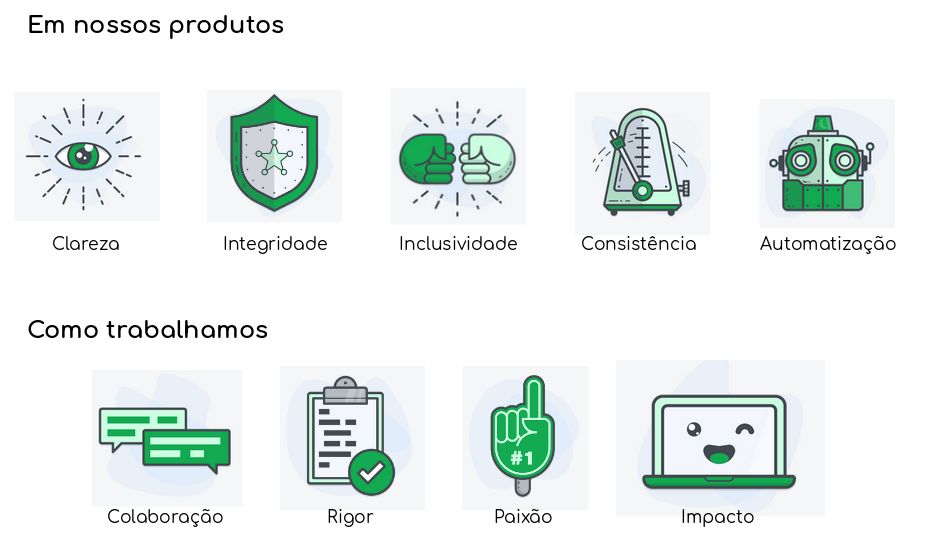
\includegraphics[width=\linewidth]{./04-figuras/02_referencial_teorico/mongodb-design-principles.png}
	\caption{Princípios de \textit{design} da Mongodb}
  \label{fig:mongodbDesignPrinciples}
\end{figure}

\begin{quadro}[!htb]
	\centering
	\begin{tabular}{|m{2cm}|m{12cm}|} \hline
		
		\multicolumn{1}{|c|}{\bfseries Princípio de \textit{Design}} & \multicolumn{1}{c|}{\bfseries Descrição} \\\hline
		
		 Clareza & Através do uso de padrões familiares, fluxos de trabalho guiados, instruções em linha e informações contextuais, nossos produtos são compreendidos sem a necessidade de um manual, quando possível, e fornecem acesso fácil à documentação concisa e clara onde necessário. A terminologia é cuidadosamente considerada e mapeia de perto o propósito ou conceito que descreve. \\\hline
		 
		 Integridade & As informações comunicadas ao usuário são precisas e completas. A transparência total instiga confiança na resiliência e segurança do produto, o que é crucial para o gerenciamento de infraestrutura crítica \\\hline
		 
		 Inclusividade & Nossos produtos atendem a todos, desde iniciantes que aprendem a usar o MongoDB pela primeira vez para especialistas na área. Quando um iniciante se sente preso, o produto fornece orientação. Quando um especialista deseja um atalho ou recurso avançado, o produto o fornece exatamente como o usuário esperaria. \\\hline
		 
		 Consistência & Os padrões de informação e interação que aparecem em diferentes lugares são consistentes visualmente e conceitualmente. Isso permite que os usuários movam-se com fluidez através de nossos produtos, confiantes de que o que aprenderem em um deles será transferido para todos os outros. \\\hline
		 
		 Automatização & Nossos produtos transmitem uma compreensão de que, às vezes, o melhor design é invisível para o usuário. Quando automatizamos uma tarefa, reduzimos a chance de erro do usuário, levando a uma experiência geral mais segura. Nossos produtos automatizam quando possível, deixando o controle com o usuário quando necessário \\\hline
		 
		 Colaboração & Reconhecemos que o melhor trabalho vem da colaboração diligente. Trabalhamos lado a lado com outros designers, engenheiros e gerentes de produto. \\\hline
		 
		 Rigor & Não estamos satisfeitos com nossas soluções até que as testamos e comprovamos sua eficácia. Nós validamos idéias e conceitos no início do processo de design, antes que qualquer \textit{wireframing} ocorra. Dados é o que nos guia. \\\hline
		 
		 Paixão & Somos intensamente apaixonados pelo nosso trabalho. Nós nos esforçamos para um nível de excelência que encanta o usuário. Mesmo detalhes aparentemente imperceptíveis recebem atenção especial. \\\hline
		 
		 Impacto & Valorizamos o impacto nas nossas entregas. Reconhecemos que nossas ferramentas e processos, enquanto evoluindo e melhorando constantemente, são apenas um meio de alcançar resultados positivos para o usuário. \\\hline
			
	\end{tabular}
	\caption{Princípios de \textit{design} da Mongodb}
	\label{table:mongodbDesignPrinciples}
	\end{quadro}

Por outro lado, a Pluralsight, uma das maiores plataformas de cursos online de tecnologia da atualidade, definiu seus princípios de forma a guiar a maneira como se comunica com seu público alvo. A \autoref{fig:pluralsightDesignPrinciples} detalha tais princípios.

\begin{figure}
	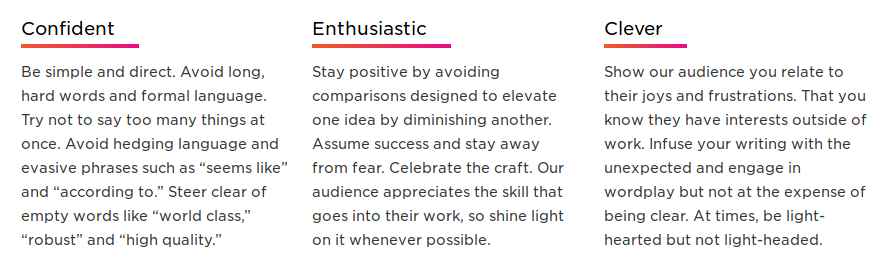
\includegraphics[width=\linewidth]{./04-figuras/02_referencial_teorico/pluralsight-principles.png}
	\caption{Princípios de \textit{design} da Pluralsight}
	\fonte{\citeonline{pluralsightDesignPrinciples}}
  \label{fig:pluralsightDesignPrinciples}
\end{figure}

Percebe-se, dados os dois exemplos apresentados, que a abordagem adotada pelas empresas na definição dos seus princípios pode variar. Não existe consenso em qual aspecto a organização deve focar. Cada empresa tem seu próprio contexto e cabe a ela aplicar os princípios da melhor maneira possível \cite{kholmatova2017design}.

Princípios de \textit{design} devem ser relacionáveis uns aos outros, fáceis de se lembrar e limitados em número. Em contrapartida, devem ser específicos o suficiente para serem capazes de auxiliarem os designers a tomarem decisões e julgar opções de maneira consistente \cite{kholmatova2017design}.

\subsection{Tom de voz}
\label{subsec:tomVoz}

No domínio verbal, os guias de tom de voz ajudam a definir a maneira com que uma organização se comunica com seu público alvo \cite{ruissalo2018operating}.

De acordo com \cite{impactOfVoiceTone}, o tom de voz tem grande impacto na percepção de confiabilidade, amigabilidade e desejo dos usuários em relação aos produtos e serviços de uma empresa. Dado que grandes organizações podem ter vários times internos, uma guia de tom de voz é fundamental para dar diretriz aos times, de forma a garantir uma comunicação coesa e consistente entre a empresa e seus clientes. \cite{impactOfVoiceTone} categoriza o tom de voz em quatro dimensões: engraçada \textit{vs} séria, casual \textit{vs} formal, insolente \textit{vs} respeitosa, entusiástica \textit{vs} objetiva.

A Firefox, empresa que mantém um navegador para internet como produto, utilizou a categorização proposta por \cite{impactOfVoiceTone}. Como pode ser visto pelas figuras \ref{fig:firefoxVoiceToneSerious} e \ref{fig:firefoxVoiceTonePlayful}, existem diferenças na maneira como a empresa se comunica com seus usuários dependendo das circunstâncias. Para situações onde ajudar o usuário é prioridade, como em casos de erros, o tom de voz é mais sério. Por outro lado, em situações onde o objetivo é motivar o usuário a tomar alguma ação -- como \textit{onboarding}, sincronização de dados ou \textit{login} -- o tom de voz é mais descontraído, não deixando de ser respeitoso.

\begin{figure}
	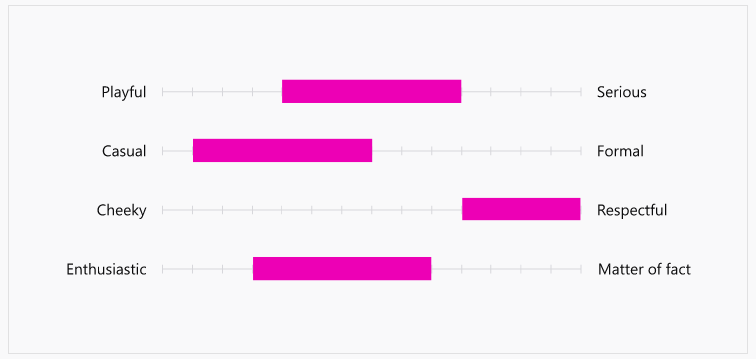
\includegraphics[width=\linewidth]{./04-figuras/02_referencial_teorico/firefox-tone-voice-01.png}
	\caption{Tom de voz para mensagens de suporte críticas da Firefox}
	\fonte{\citeonline{firefoxVoiceTone}}
  \label{fig:firefoxVoiceToneSerious}
\end{figure}

\begin{figure}
	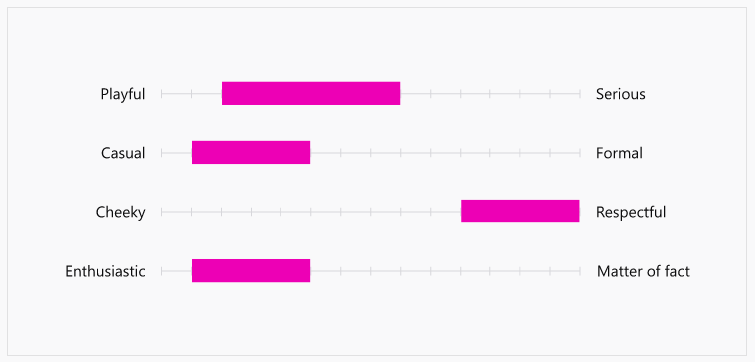
\includegraphics[width=\linewidth]{./04-figuras/02_referencial_teorico/firefox-tone-voice-02.png}
	\caption{Tom de voz para mensagens motivacionais da Firefox}
	\fonte{\citeonline{firefoxVoiceTone}}
  \label{fig:firefoxVoiceTonePlayful}
\end{figure}

\subsection{Biblioteca de componentes}
\label{sec:bibliotecaComponentes}

Desde a concepção das interfaces de usuário (GUI), a relevância da consistência nas interfaces através dos diferentes produtos de uma organização foi percebida imediatamente \cite{ruissalo2018operating}. Para sanar esse problema, foi proposta a definição das chamadas bibliotecas de componentes. A \autoref{fig:bootstrapStyleGuide} apresenta um exemplo de biblioteca de componentes muito utilizada pela indústria: Bootstrap.

As bibliotecas de componentes tradicionais eram focadas em padronizar o uso dos componentes do produto, como tipografia, imagens e ilustrações, cores, \textit{layouts} e outros elementos gráficos \cite{ruissalo2018operating}. Eram, portanto, focadas somente nos aspectos visuais das aplicações, definindo o que era esperado a ser apresentado para o usuário final.

De acordo com \cite{taylor2007software}, \textit{design} no contexto de desenvolvimento de software está mais diretamente ligado na arquitetura dos produtos ao invés de uma mero padrão de estilização. Essa é a razão pela qual o \textit{design} pode, e deve, estar mais próximo da implementação do \textit{software}. Tal abordagem vai de encontro com um antigo dogma: guias de estilo e bibliotecas de componente são propriedade dos \textit{designers} \cite{ruissalo2018operating}. Espera-se que as bibliotecas de componentes sejam o resultado do trabalho conjunto de \textit{designers} e desenvolvedores.

\begin{figure}
	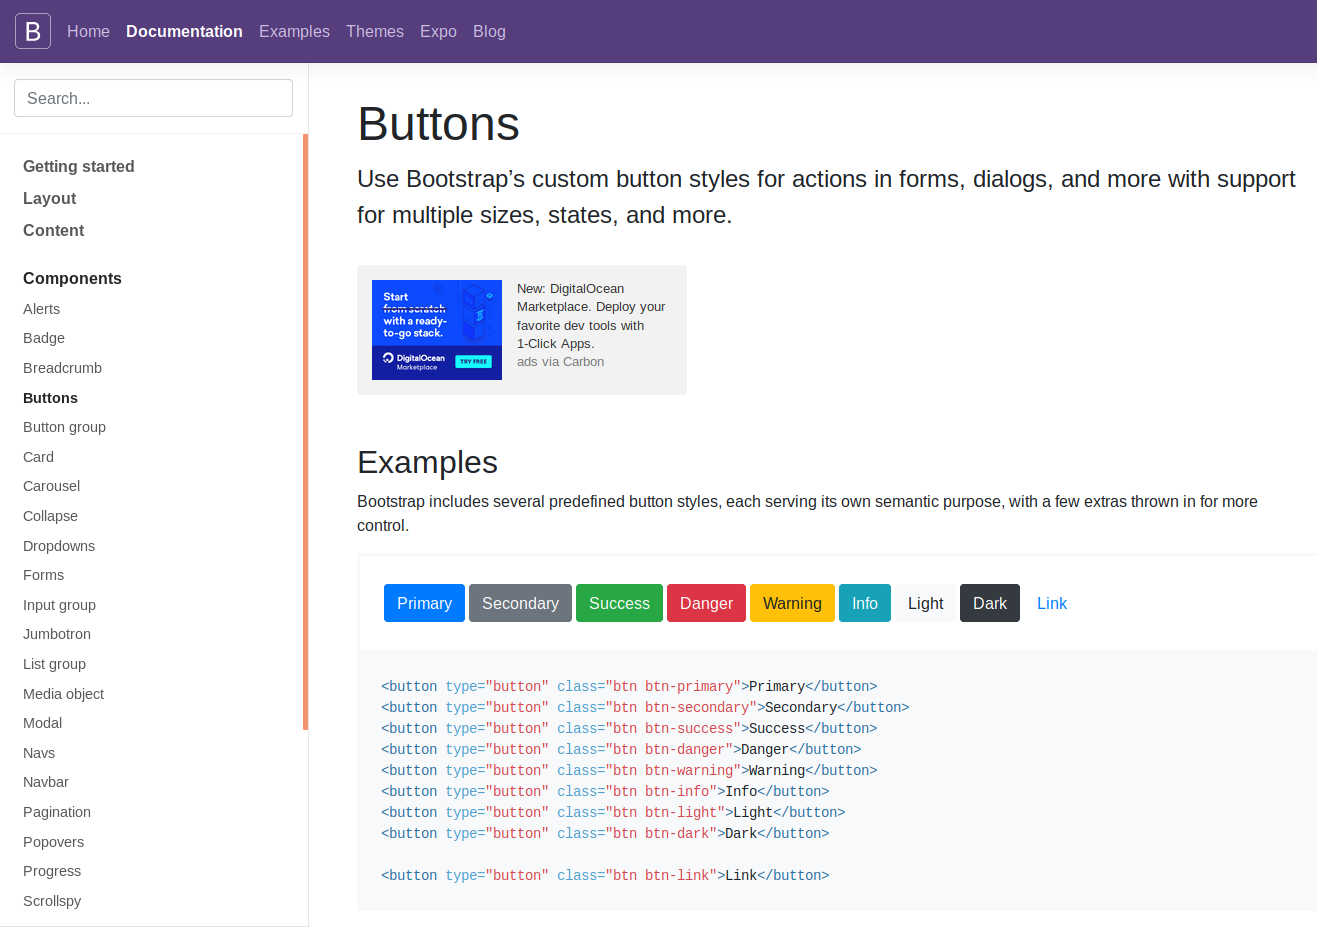
\includegraphics[width=\linewidth]{./04-figuras/02_referencial_teorico/bootstrap.png}
	\caption{Exemplo de biblioteca de componentes}
	\fonte{\citeonline{bootstrapStyleGuide}}
  \label{fig:bootstrapStyleGuide}
\end{figure}

\section{\textit{Atomic Design}}
\label{sec:atomicDesign}

Conforme apresentado na seção anterior, \textit{Design Systems} se propõem a revolucionar a forma como se constroi interfaces de usuário à nível profissional. Entretanto, a forma como são apresentados seus conceitos é, em geral, um tanto quanto subjetiva, ficando a cargo de cada instituição definir a melhor abordagem para o seu problema. Para o caso das bibliotecas de componentes em especial, tanta liberdade assim poderia acarretar em problemas de escalabilidade da solução.

Com o intuito de definir uma metodologia para a implementação técnica de um \textit{Design System}, \cite{frostAtomicDesign} buscou na química inspiração para a resolução do problema. A idéia residia no fato de que toda matéria -- seja sólida, líquida, gasosa, simples, complexa, etc -- é composta por unidades minúsculas e indivisíveis (ou quase) chamadas átomos. Tais átomos, combinados entre si formam unidades mais complexas, conhecidas como moléculas. Essas, por sua vez, combinadas formas estruturas ainda mais complexas chamadas organismos. E assim é expressa toda a mateŕia do universo.

Analogamente à matéria, interfaces de usuários também podem ser expressas por componentes menores. Isso significa que é possível construir interfaces bastante complexas através de um conjunto de componentes menores e mais simples. A \autoref{fig:periodicTable} ilustra e categoriza elementos HTML a níveis atômicos.

\begin{figure}
	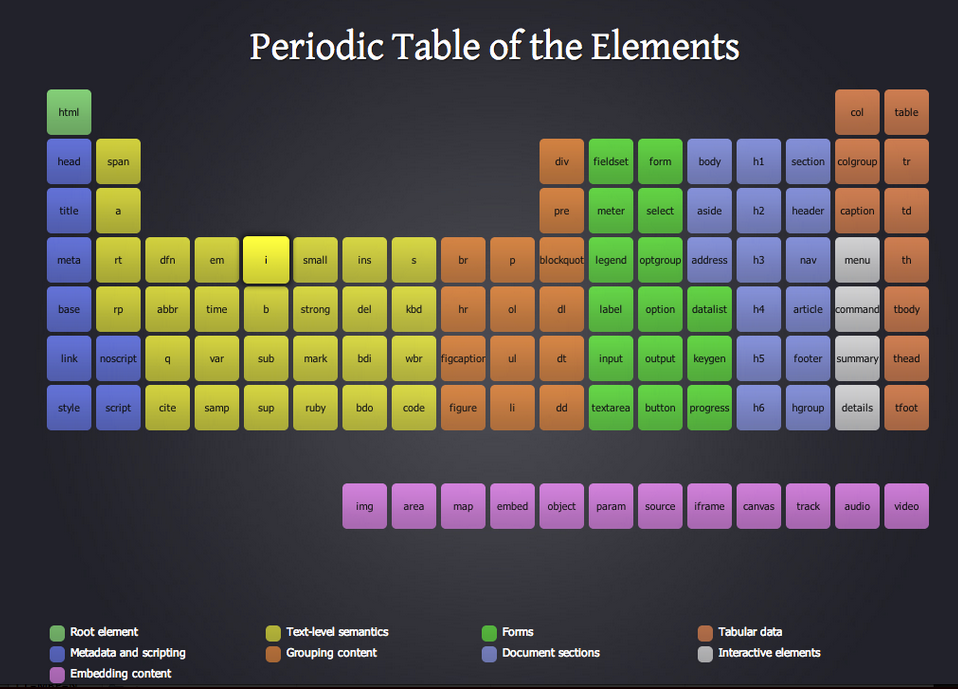
\includegraphics[width=\linewidth]{./04-figuras/02_referencial_teorico/periodic-table.png}
	\caption{Tabela períodica de elementos HTML proposta por Josh Duck}
	\fonte{\citeonline{frostAtomicDesign}}
  \label{fig:periodicTable}
\end{figure}

Dessa forma, \cite{frostAtomicDesign} defende a existência de cinco níveis distintos no \textit{Atomic Design}: Átomos, Moléculas, Organismos, Templates e Páginas. A \autoref{fig:atomicDesignLevels} ilustra tais níveis e a forma como eles comunicam entre si.

\begin{figure}
	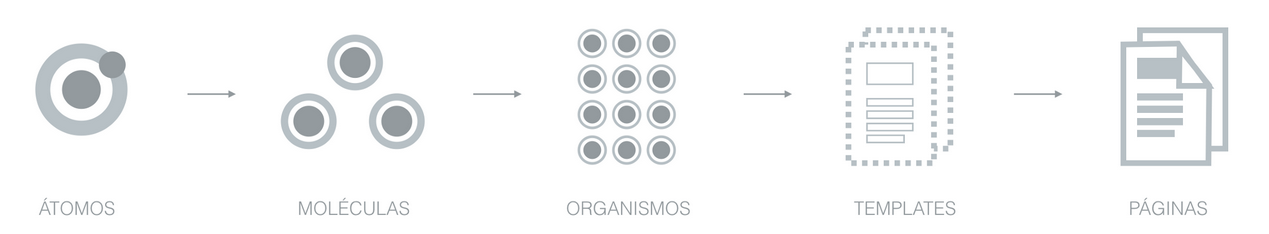
\includegraphics[width=\linewidth]{./04-figuras/02_referencial_teorico/atomic-levels.png}
	\caption{Níveis do \textit{Atomic Design}}
	\fonte{\citeonline{frostAtomicDesign}}
  \label{fig:atomicDesignLevels}
\end{figure}

\subsection{Átomos}
\label{subsec:atomos}

Átomos são os blocos básicos para construção da matéria. Aplicados no universo de interfaces de usuário Web, átomos são as \textit{tags} HTML, como um \textit{input}, botão, \textit{label}, etc.

Assim como os átomos da natureza, eles não são muito úteis de serem manipulados individualmente. Entetanto, cumprem um papel fundamental na construção da biblioteca de componentes, uma vez que todos os componentes mais complexos do sistema são construídos com base neles.

\subsection{Moléculas}
\label{subsec:moleculas}

Tudo começa a ficar mais tangível quando combinamos átomos. As moléculas são um conjunto de átomos distintos que ficam encapsulados juntos. São a espinha dorsal de todo o \textit{Design System}.

Por exemplo, um \textit{label}, um botão e um \textit{input} individualmente não são muito úteis para o usuário final, porém juntos eles formam um formulário que pode de fato gerar valor para o interlocutor.

Construir moléculas a partir de átomos estimula os desenvolvedores a seguir a mentalidade de "faça uma vez, mas faça direito" \cite{frostAtomicDesign}.

\subsection{Organismos}
\label{subsec:organismos}

Organismos são grupos de moléculas que juntas formam uma seção relativamente complexa e distinta da interface de usuário. Examplos de organismos poderiam ser: o cabeçalho de uma página, a seção de menu, etc.

Como organismos já estão em um nível bastante concreto, conseguem definir a estrutura da interface do usuário com bastante clareza. São comumente utilizados como base para uma conversa com clientes finais de um dado produto, uma vez que conseguem transmitir a idéia de valor de uma funcionalidade.

Construir organismos a partir de moléculas estimula os desenvolvedores a construir componentes portáveis e reusáveis \cite{frostAtomicDesign}.

\subsection{Templates}
\label{subsec:templates}

Chegando no nível de templates, abre-se mão da analogia à química para se valorizar uma linguagem que faça mais sentido para os clientes da aplicação. Templates consistem em um conjunto de organismos que compõem uma página. Aqui, começa-se a visualizar o resultado final do \textit{design}, podendo-se visualizar o \textit{layout} em ação.

A \autoref{fig:atomicDesignTemplate} apresenta um exemplo de um possível template em um \textit{Atomic Design}.

\begin{figure}
	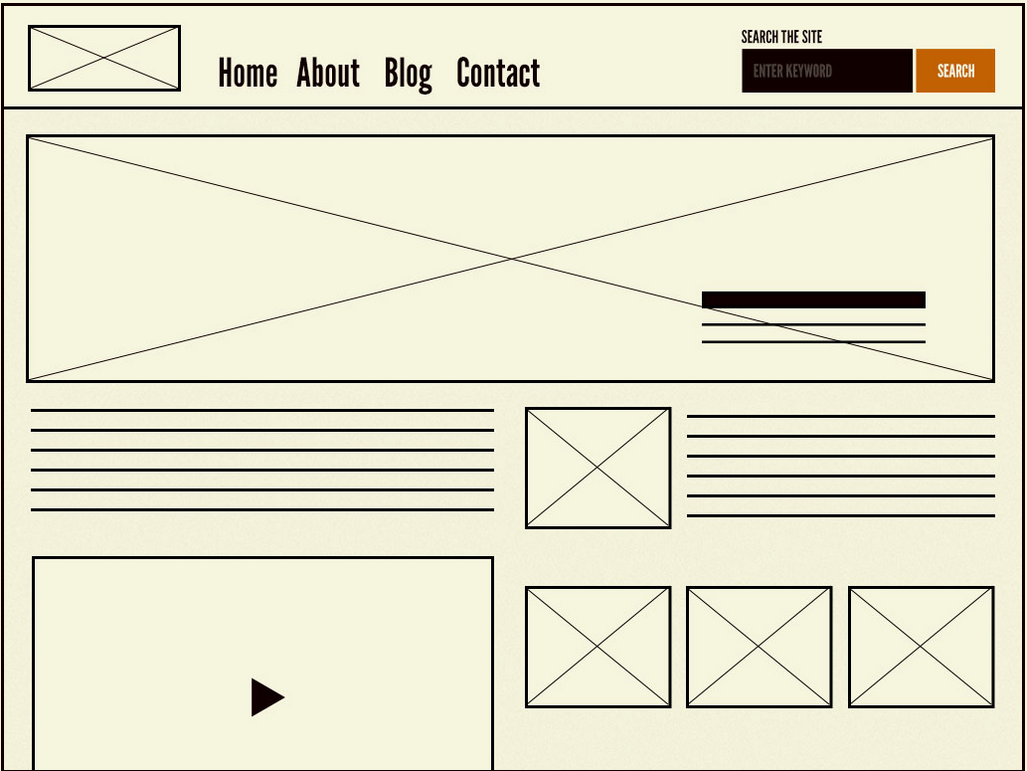
\includegraphics[width=\linewidth]{./04-figuras/02_referencial_teorico/ad-template.png}
	\caption{Exemplo de template}
	\fonte{\citeonline{frostAtomicDesign}}
  \label{fig:atomicDesignTemplate}
\end{figure}

\subsection{Páginas}

Páginas são instâncias específicas de um dado template. Nesse momento, conteúdos de marcação são substituídos por valores reais a serem utilizados na interface de usuário.

Esse estágio é crucial pois é nele onde se testa a efetividade do \textit{design system}. Visualizando todos componentes em um mesmo ambiente facilita o trabalho de validar e eventualmente modificar algum átomo, mólecula, organismo ou template, de forma a atingir melhores resultados.
  % Fundamentação teórica
% -----------------------------------------------------------------------------
% Trabalhos Relacionados
% -----------------------------------------------------------------------------

\chapter{Trabalhos Relacionados}
\label{chap:trabRelac}

Cada capítulo deve conter uma pequena introdução (tipicamente, um ou dois parágrafos), em seção não numerada, que deve deixar claro o objetivo e o que será discutido no capítulo, bem como a organização do capítulo.
 % Trabalhos relacionados
% -----------------------------------------------------------------------------
% Metodologia
% -----------------------------------------------------------------------------

\chapter{Metodologia}
\label{chap:metodologia}
Cada capítulo deve conter uma pequena introdução (tipicamente, um ou dois parágrafos), em seção não numerada, que deve deixar claro o objetivo e o que será discutido no capítulo, bem como a organização do capítulo.

\section{Delineamento da pesquisa}
\label{sec:titSecDelPesq}

Inserir seu texto aqui...

\section{Coleta e tratamento de dados}
\label{sec:titSecColDad}

Inserir seu texto aqui...

            % Metodologia
% -----------------------------------------------------------------------------
% Entrevistas com Stakeholders
% -----------------------------------------------------------------------------

\chapter{Entrevistas com \textit{Stakeholders}}
\label{chap:entrevistas}


Como forma de validar a real necessidade de criação de um \textit{design system} na empresa avaliada no experimento, foram realizadas entrevistas com os principais \textit{stakeholders} do projeto: designers e desenvolvedores \textit{frontend}. Neste capítulo são apresentados, de maneira consolidada, os resultados obtidos como consequência de tais entrevistas.

Para garantir que os resultados não fossem enviezados em um único contexto da organização, foram selecionados 3 profissionais com desafios destintos dentro da empresa, como representantes de cada um dos grupos.

Todas as entrevistas foram gravadas, conforme conscentimento dos participantes. Para garantir o anônimato dos envolvidos, todos os dados apresentados neste capítulo estarão associados a nomes de marcação, não expondo nomes e dados pessoais reais dos voluntários.

\section{Designers}
\label{sec:entrevistasDesigners}

De acordo com o roteiro de entrevista ilustrado no Apêndice A deste projeto, os designers avaliados foram submetidos a algumas perguntas genéricas onde puderam expor um pouco dos detalhes do seu dia-a-dia de trabalho. O \autoref{table:designersResearch} apresenta as características de cada um dos profissionais entrevistados.

\begin{quadro}
\centering
\begin{tabular}{|m{4cm}|m{10cm}|} \hline
	
	\multicolumn{1}{|c|}{\bfseries Voluntário} & \multicolumn{1}{c|}{\bfseries Contexto} \\\hline
	
	 Designer 1 & Profissional mais experiente do grupo, sendo a principal referência de design em toda a organização. Está diretamente envolvido em um projeto mais novo e bastante promissor da empresa. Nesse projeto, teve a liberdade de definir novos padrões de design que hoje são tomados como referência para todos os novos produtos da empresa. \\\hline
	 
	 Designer 2 & Pilar de design do maior \textit{squad} da empresa, que tem como objetivo dar manutenção e evoluir todo o fluxo de comunicação da plataforma. Está diretamente envolvido com sistemas legados do produto, e tem como principal desafio garantir uma boa experiência do usuário ao longo do uso da plataforma. \\\hline
	 
	 Designer 3 &  Responsável pelo design da área de marketing da organização, estando diretamente envolvido em campanhas de eventos, contratação e lançamento de novos produtos. Também é responsável pelas artes do site e do blog de tecnologia da empresa. \\\hline
    
\end{tabular}
\caption{Características dos designers entrevistados}
\fonte{Próprio autor}
\label{table:designersResearch}
\end{quadro}

A seguir, são apresentados os resultados consolidados de perguntas chave realizadas nas entrevistas.

\textbf{Questão 1:} Contextualize, brevemente, a maneira como os processos de design são adotados na empresa, atualmente.

\begin{quote}
    A maioria das empresas de tecnologia são focadas no desenvolvedor. Por isso, grande parte dos processos de desenvolvimento existentes estão associados ao código-fonte, sendo o design muitas vezes negligenciado. Por muito tempo essa foi a realidade da Dito, porém nos últimos 2 anos a área de design começou a conquistar seu espaço na organização, tendo, pela primeira vez, profissionais especializados da área designados a evoluírem a plataforma com foco no usuário final do produto.
    
    Foi a partir desse momento que iniciaram-se trabalhos para definir os primeiros processos de design da empresa. O primeiro deles foi a inclusão de ferramentas como Sketch e Zeplin na rotina dos designers e desenvolvedores \textit{frontend}. Com elas, o designer exerce seu papel de pensar na melhor interface de usuário possível para um dado problema e, após sua prototipação, o desenvolvedor tem acesso a arte de maneira detalhada tecnicamente. Isso fez com que as novas interfaces desenvolvidas, desde então, fossem mais fidedignas àquilo idezaliado pelo designer.
    
    Apesar do considerável avanço, ainda entende-se que a empresa está "engatinhando" no que se diz respeito à processos de design. Ainda existe uma visão geral de que design se restringe unicamente à criação de interfaces. No que se tange à concepção de produtos, não está bem definido um processo de design escalável. Pensando nisso, um dos \textit{squads} da empresa vem tentando implacar um novo modelo conhecido como \textit{Double Diamond Design}, proposto pela metodologia de \textit{design thinking}. Tal processo é dividido em fases de imersão, ideação, prototipação e testes de usabilidade, objetivando a construção de produtos de maneira mais rápida e aderente às necessidades do usuários final.
    
    Na área de marketing, por sua vez, o contexto é um pouco diferente: contando apenas com dois profissionais alocadas para gerenciar toda a área, a criação de uma \textit{styleguide} se tornou uma necessidade latente. A maneira encontrada para se ganhar velocidade, e atender à toda a demanda da empresa, foi a criação de templates. Tal \textit{styleguide} foi criada a partir de um dos produtos da plataforma, porém não existe ligação alguma entre os dois artefatos.
\end{quote}

\textbf{Questão 2:} Quais as maiores dificuldades e frustrações que você encontra no seu trabalho, como consequência dos processos atuais de design?

\begin{quote}
    Tendo em vista que a maturidade em design da Dito está passando por um processo de evolução, os designers da empresa ainda precisam empregar uma quantidade de esforço significativa para a construção de novos protótipos de interfaces de usuários, uma vez que a capacidade de reusabilidade de componentes ainda está aquém do ideal. 
    
    Por conta disso, as maiores frustrações do time, em geral, estão relacionadas à impossibilidade de se ter um contato mais próximo com o usuário final do produto. Deseja-se que tarefas de teste de usabilidade e metrificação de maturidade façam parte do processo de design da Dito, porém atualmente isso é inviável pois os designers estão muito ocupados em dar vazão à demandas de criação de novas interfaces.
    
    Também destaca-se a falta de uma figura exclusivamente responsável por definir e garantir que as diretrizes de design estão sendo seguidas pela organização como um todo. Espera-se que essa pessoa também exerça o papel de tutor de talentos menos experientes, papel este inexistente na conjuntura atual da empresa.
\end{quote}

\textbf{Questão 3:} Como são tomadas decisões de design na empresa? E no seu time? Quem são as pessoas envolvidas?

\begin{quote}
    Basicamente, a partir da apresentação de um dado desafio, inicia-se uma fase de análise aprofundada do problema. Durante essa fase, é bastante comum o envolvimento de profissionais de negócio e desenvolvedores para a validação da viabilidade de possíveis soluções. Vez ou outra acontecem alterações nas decisões de design pré-estabelecidas devido à inviabilidade técnica da proposta. Portanto, esse tipo de tomada de decisão já é fruto de um trabalho colaborativo entre diferentes perfis de profissionais.
    
    Entretanto, o núcleo das discussões normalmente acontece no contexto individual do \textit{squad} responsável pelo problema. Não existe consenso geral de diretrizes a serem seguidas pelos times. Dessa forma, o cenário atual é caracterizado pelo trabalho isolado dos designers da empresa. Cada um deles se mantém focado exclusivamente nos desafios do seu próprio \textit{squad}, não sendo comum um intercâmbio de experiências entre os membros da área de design como um todo.
    
    Foram levantadas, ainda, situações em que decisões de design foram tomadas por profissionais de negócio, mesmo quando em desacordo do ponto de vista do designer responsável pela entrega. Devido à falta de autoridade da área, sendo um claro reflexo da imaturidade da mesma, a experiência do usuário acaba sendo prejudicada em detrimento do cumprimento de prazos estabelecidos para entregas.
\end{quote}

\textbf{Questão 4:} Como você classifica a velocidade de desenvolvimento de novas interfaces de usuários atualmente? Por que?

\begin{quote}
    De maneira geral, está mais rápida do que o observado em momentos anteriores à definição dos processos inicias de design, porém poderia estar melhor caso existisse uma biblioteca de componentes bem estruturada.
\end{quote}

\textbf{Questão 5:} Você acredita que um \textit{design system} poderia ser uma opção plausível para alavancar a capacidade de escalabilidade do produto da empresa?

\begin{quote}
    De maneira unânime, sim.

    A padronização de ferramentas e processos é, sem dúvidas, um excelente promotor do potencial de escalabilidade do produto. Estima-se que, com uma biblioteca de componentes bem estruturada, tarefas de prototipação seriam executadas 4 vezes mais rapidamente.
    
    Entende-se, entretanto, que a criação de um \textit{design system} é um projeto bastante ambicioso e complexo, fazendo-se necessário o envolvimento, preferencialmente exclusivo, de uma série de profissionais com nível avançado de senioridade. O resultado final do projeto é um artefato que tem a pretenção de resolver problemas de comunicação de toda uma organização, portanto sua concepção deve ser embasada nas dores de todos os grupos que compõem a empresa.
    
    Ressalta-se ainda que, o processo de criação de um \textit{design system} deve ser encarado como um produto e não um projeto. Para tanto, o mesmo deve estar em constante evolução, mantendo sua documentação viva e atualizada.
\end{quote}

\section{Desenvolvedores \textit{frontend}}
\label{sec:entrevistasDevs}

De acordo com o roteiro de entrevista ilustrado no Apêndice B deste projeto, os desenvolvedores avaliados foram submetidos a algumas perguntas genéricas onde puderam expor um pouco dos detalhes do seu dia-a-dia de trabalho. O \autoref{table:devsResearch} apresenta as características de cada um dos profissionais entrevistados.

\begin{quadro}
\centering
\begin{tabular}{|m{4cm}|m{10cm}|} \hline
	
	\multicolumn{1}{|c|}{\bfseries Voluntário} & \multicolumn{1}{c|}{\bfseries Contexto} \\\hline
	
	 Desenvolvedor 1 & Profissional que teve mais contato com a base de código-fonte da plataforma. Com mais de 4 anos de colaboração com o produto, teve a oportunidade de participar de vários projetos da empresa. Atualmente, assume o desafio de liderança do \textit{squad} de suporte técnico da organização. \\\hline
	 
	 Desenvolvedor 2 & Principal desenvolvedor do \textit{squad} responsável por manter um dos mais recentes e promissores produtos da empresa. Nesse projeto, teve a oportunidade de trabalhar com tecnologias mais inovadoras do que aquelas utilizadas na base de código-fonte legada da plataforma. \\\hline
	 
	 Desenvolvedor 3 & Mais novo colaborador do \textit{squad} de comunicação da empresa. Está a cerca de 2 meses assumindo o desafio de manter e evoluir sistemas legados de \textit{fronted} da plataforma. \\\hline
    
\end{tabular}
\caption{Características dos desenvolvedores entrevistados}
\fonte{Próprio autor}
\label{table:devsResearch}
\end{quadro}

A seguir, são apresentados os resultados consolidados de perguntas chave realizadas nas entrevistas.

\textbf{Questão 1:} Contextualize, brevemente, a maneira como os processos de desenvolvimento \textit{frontend} são adotados na empresa, atualmente.

\begin{quote}
    Em momentos anteriores à definição dos primeiros processos de design, era papel do desenvolvedor definir e implementar as interfaces de usuário. Não havia nenhuma atividade de pesquisa e validação com os usuários finais.
    
    A partir de então, especificações de páginas web já vêm sendo realizadas por profissionais especializadas e compartilhadas com o desenvolvedor por meio de ferramentas como Sketch e Zeplin. Percebeu-se, como consequência da adoção de tais ferramentas e processo, uma considerável melhoria na velocidade de desevolvimento e da qualidade final das telas.
    
    Após a implementação das interfaces, inicia-se uma fase de validação do artefato em um ambiente controlado chamado de \textit{staging}. Nesse ambiente, o designer certifica-se de que o foi produzido está realmente de acordo com suas especificações.
    
    Caso aprovado, o código-fonte produzido é incorporado à plataforma e começa a gerar valor para o usuário final.
\end{quote}

\textbf{Questão 2:} Quais as maiores dificuldades e frustrações que você encontra na plataforma durante o desenvolvimento de suas atividades?

\begin{quote}
    A maioria das frustrações apresentadas pelos voluntários residem na atual estrutura do principal produto da empresa, conhecido como \textit{dashboard}. Trata-se de um projeto legado, que teve o início de sua construção iniciado à cerca de 7 anos atrás e que utiliza uma \textit{stack} tecnológica atualmente bastante defasada.
    
    Como consequência da sua arquitetura degrada e pela falta de testes de interface no projeto, existe grande receio em se realizar alterações em alguns componentes, pois abre-se a possibilidade de ocorrência de efeitos colaterais inesperados e catastróficos. Por conta disso, é bastante comum encontrarmos diferentes soluções para um mesmo problema. Existe muito código-fonte duplicado ao longo do projeto.
    
    Não existe, ainda, nenhuma biblioteca de componentes bem definida que facilite o reuso de soluções já implementadas e padronize a forma como se constrói novas interfaces de usuário.
\end{quote}

\textbf{Questão 3:} Como você classifica a velocidade de desenvolvimento de novas interfaces de usuários atualmente? Por que?

\begin{quote}
    Está aquém do ideal. Tarefas de desenvolvimento \textit{frontend} são, em geral, bastante custosas de serem realizadas. Atividades que deveriam ser simples de serem executadas, normalmente não são.
    
    É necessário adquirir-se certa fluência com a estrutura e deficiências do projeto. Só assim é possível atingir uma velocidade de desenvolvimento satisfatória. Em geral, o tempo para se atingir tal fluência não é curto, muito por conta da complexidade da base de código-fonte da plataforma e do uso de uma \textit{stack} tecnológica defasada.
\end{quote}

\textbf{Questão 4:} De modo geral, como você classifica a atual arquitetura frontend da plataforma a nível de escalabilidade e reusabilidade?

\begin{quote}
    Levando em consideração a capacidade de escalabilidade do produto, houveram respostas contraditórias, uma vez que as mesmas foram embasadas em perspectivas distintas à respeito da arquitetura.
    
    Em um primeiro momento, foi levantado que a arquitura é escalável, pois o padrão MVC proposto pelo \textit{framework} utilizado na plataforma proporciona tal fenômeno. \textit{Frameworks} que oferecem mais flexibilidade na maneira como se organiza o projeto, podem contribuir para a construção de arquiteturas pouco escaláveis, uma vez que podem não existir padrões bem definidos no projeto como um todo.
    
    Em contrapartida, existe também a visão de que a plataforma é pouco escalável, pois há um forte acoplamento entre o \textit{backend} e o \textit{frontend}. A renderização das interfaces de usuários acontecem, muitas vezes, de maneira mista: parte acontece no universo \textit{frontend} e a outra parte no \textit{backend}. Esse tipo de exemplo de inconsistência é um fator recorrente em toda a plataforma, o que prejudica seu potencial de escalabilidade.
    
    No quesito reusabilidade, o parecer foi unânime. A plataforma é pouco reusável, apresentando várias ocorrências de duplicidade de código-fonte como alternativa para se evitar efeitos colaterais em cenários alternativos.
\end{quote}

\textbf{Questão 5:} Você já ouviu falar no termo \textit{design system}? Se sim, acredita que poderia ser uma abordagem plausível para impulsinar a capacidade de escalabilidade do produto da empresa?

\begin{quote}
    Novamente, de maneira unânime, sim.

    Para se trabalhar em uma plataforma que cresce em velocidade recorde ano após ano, a existência de um \textit{design system} é fator fundamental para atingir as expectativas de velocidade aumejadas pela organização.
    
    Entretando, assim como o observado pelos designers, entende-se que a criação de um \textit{design system} completo é uma tarefa árdua. Necessita-se de profissionais qualificados e que estejam realmente focados em construir uma ferramenta tão ambiciosa assim.
    
    Para se mitigiar o fênomeno da degradação e defasamento das tecnologias adotadas, idealiza-se a contrução de uma bilbioteca de componentes de maneira desacoplada de tecnologias ou frameworks específicos. O ideal seria construir a biblioteca de componentes baseados nos chamados \textit{Web Components}. Dessa forma, migrações de tecnologias defasadas para tecnologias mais recentes acontecerão de maneira menos traumática, uma vez que não existe dependência alguma entre o legado e a biblioteca de componentes em si.
    
    Por fim, também foi apontada a preocupação de se manter as diretrizes expostas pelo \textit{design system} constantemente atualizadas, de forma a se evitar o seu desuso.
\end{quote}

Conforme observado pelas entrevistas, muitos dos problemas apresentados no capítulo 2 deste projeto, também se manifestam na empresa avaliada no experimento. Dada sua atual conjuntura, tal como a realidade do seu produto, a necessidade de criação de um \textit{design system} foi comprovada.

No capítulo seguinte será apresentada a biblioteca de componentes criada, em um formato de protótipo, para se iniciar o processo de surgimento do novo \textit{design system} da organização.
            % Entrevistas
% -----------------------------------------------------------------------------
% Resultados
% -----------------------------------------------------------------------------

\chapter{Análise e Discussão dos Resultados}

Cada capítulo deve conter uma pequena introdução (tipicamente, um ou dois parágrafos), em seção não numerada, que deve deixar claro o objetivo e o que será discutido no capítulo, bem como a organização do capítulo.

\section{Título da seção}
\label{sec:titSecResult}

Inserir seu texto aqui...
             % Resultados
% -----------------------------------------------------------------------------
% Conclusão
% -----------------------------------------------------------------------------

\chapter{Conclusão}
\label{chap:conclusao}

Procure fazer uma análise crítica de seu trabalho, destacando os principais resultados e as contribuições deste trabalho para a área de pesquisa.

\section{Trabalhos Futuros}
\label{sec:trabalhosFuturos}

Também deve indicar, se possível e/ou conveniente, como este trabalho pode ser estendido ou aprimorado.

\section{Considerações Finais}
\label{sec:consideracoesFinais}

As derradeiras palavras para encerramento do seu trabalho acadêmico.

% -----------------------------------------------------------------------------
% Observação: A norma ABNT estabelece que em qualquer tipo de trabalho
% acadêmico monográfico deve haver um capítulo de conclusão
% -----------------------------------------------------------------------------
              % Conclusão

% Insere os elementos pós-textuais
\postextual
% -----------------------------------------------------------------------------
% Referências
% -----------------------------------------------------------------------------

% Carrega o arquivo "referencias.bib" com as referências do trabalho
\bibliography{./referencias}{}

% Define o estilo ABNT para formatar a lista de referências
\bibliographystyle{abntex2-alf}

% -----------------------------------------------------------------------------
% Não é necessário editar este arquivo.
% -----------------------------------------------------------------------------
        % Referências
% -----------------------------------------------------------------------------
% Apêndices
% -----------------------------------------------------------------------------

\begin{apendicesenv}
\partapendices

% -----------------------------------------------------------------------------
% Primeiro apêndice
% -----------------------------------------------------------------------------

\chapter{Nome do apêndice}
\label{chap:apendiceA}

Lembre-se que a diferença entre apêndice e anexo diz respeito à autoria do texto e/ou material ali colocado.

Caso o material ou texto suplementar ou complementar seja de sua autoria, então ele deverá ser colocado como um apêndice. Porém, caso a autoria seja de terceiros, então o material ou texto deverá ser colocado como anexo.

Caso seja conveniente, podem ser criados outros apêndices para o seu trabalho acadêmico. Basta recortar e colar este trecho neste mesmo documento. Lembre-se de alterar o "label"{} do apêndice.

Não queira colocar tudo que é complementar em um único apêndice. Organize seus apêndices de modo a que, em cada um deles, haja um único tipo de conteúdo. Isso facilita a leitura e compreensão para o leitor do trabalho. É para ele que você escreve.

% -----------------------------------------------------------------------------
% Novo apêndice
% -----------------------------------------------------------------------------

\chapter{Estrutura de trabalhos acadêmicos}
\label{chap:apEstrTrabAcad}

Quanto à estrutura do trabalho acadêmico, esta varia sobremaneira, a depender da conveniência do autor e seu(s) respectivo(s) orientador(es). No entanto, de acordo com as normas ABNT, alguns elementos são obrigatórios.

A título de sugestão, e apenas isso, a \autoref{fig:estrutura-projeto-qualificacao} apresenta uma estrutura para um projeto de qualificação de mestrado ou doutorado, conforme a norma \citeonline{NBR14724:2011}.

\begin{figure}[!htb]
    \centering
    \caption{Estrutura sugerida de um Projeto de Qualificação para os cursos de Mestrado ou Doutorado}
    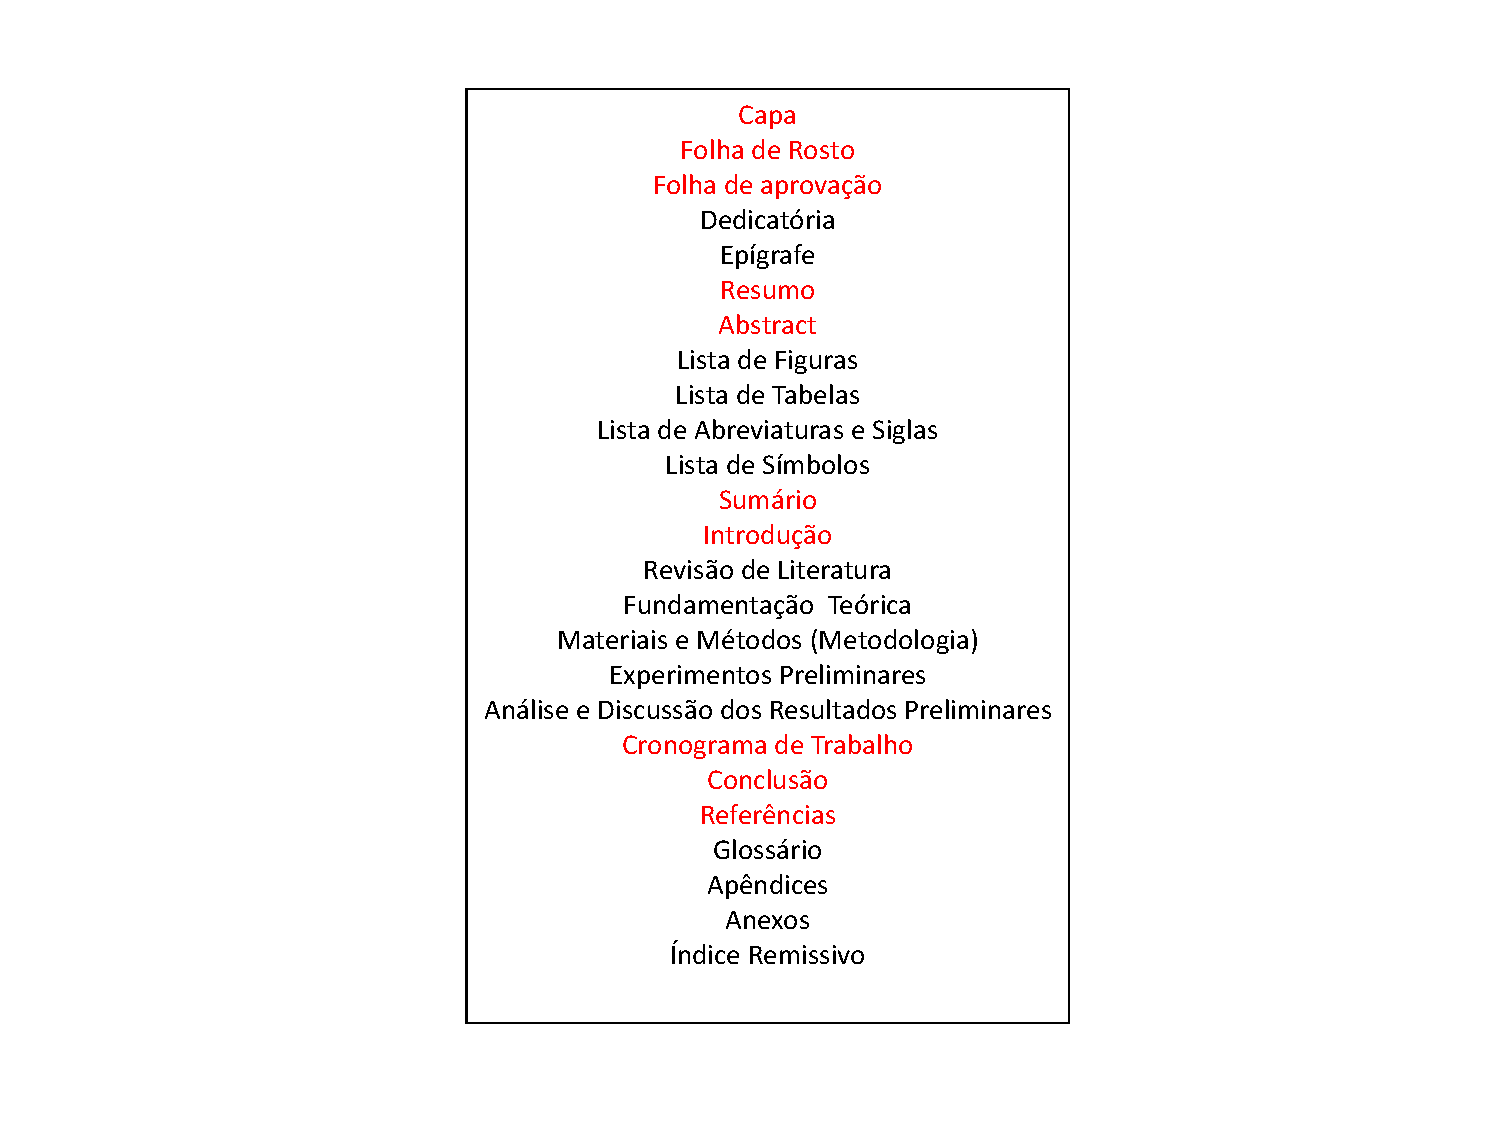
\includegraphics[width=0.5\textwidth]{./04-figuras/estrutura-projeto-qualificacao}
    \label{fig:estrutura-projeto-qualificacao}
\end{figure}

Já a \autoref{fig:estrutura-tese-dissertacao} apresenta uma estrutura para uma tese de doutorado ou dissertação de mestrado, conforme a norma \citeonline{NBR14724:2011}.

Cabe ressaltar que, em todas as figuras, os elementos obrigatórios estão destacados em vermelho, os demais são opcionais.

\begin{figure}[!htb]
    \centering
    \caption{Estrutura sugerida de uma Tese de Doutorado ou Dissertação de Mestrado}
    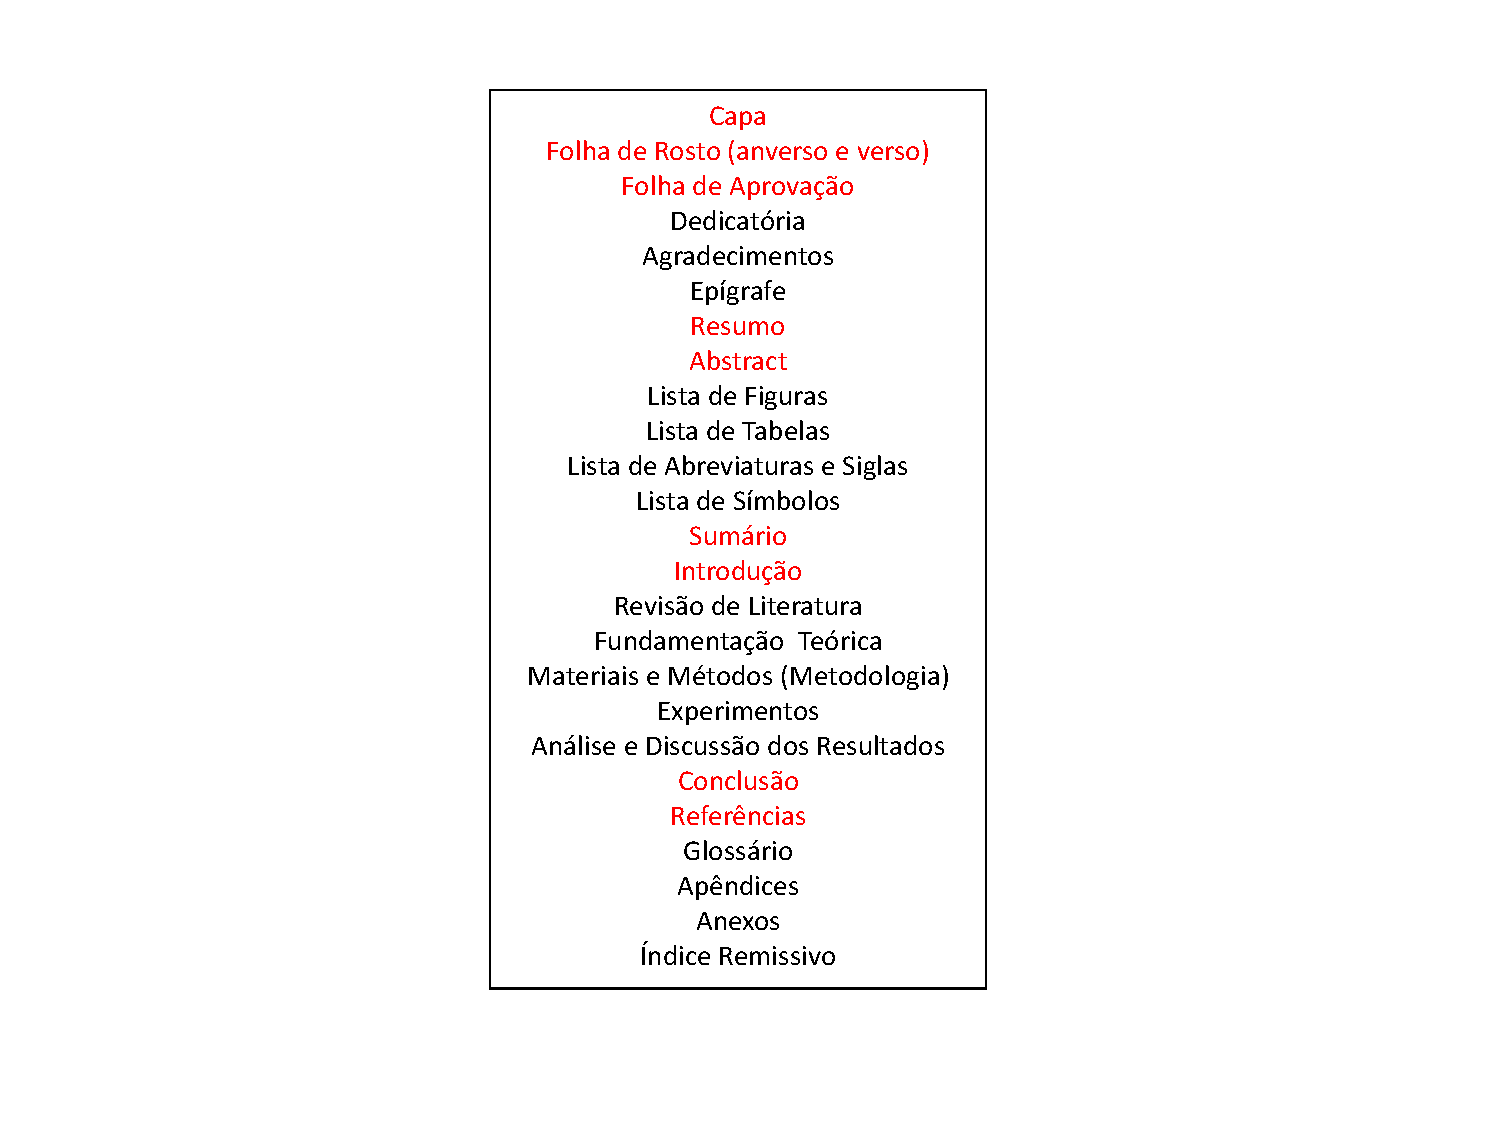
\includegraphics[width=0.5\textwidth]{./04-figuras/estrutura-tese-dissertacao}
    \label{fig:estrutura-tese-dissertacao}
\end{figure}

Observe que a estrutura de um projeto de qualificação é muito similar à da tese ou dissertação. A única diferença existente é que num projeto de qualificação o autor certamente terá, via de regra, apenas resultados parciais e preliminares. Além disso, estando o trabalho ainda em andamento, há que se apresentar um cronograma de trabalho que evidencie que o mesmo poderá ser concluído dentro dos prazos estabelecidos pelo programa.

Por fim, como foi dito, este  \emph{template} pode ser utilizado para outros trabalhos acadêmicos. Neste caso, a \autoref{fig:estrutura-projeto-pesquisa} apresenta uma sugestão de projeto de pesquisa a ser submetido ao programa para fins de admissão ao mesmo, conforme a norma \citeonline{NBR15287:2005}.

\begin{figure}[!htb]
    \centering
    \caption{Estrutura sugerida de um projeto de pesquisa para admissão ao PPGMMC}
    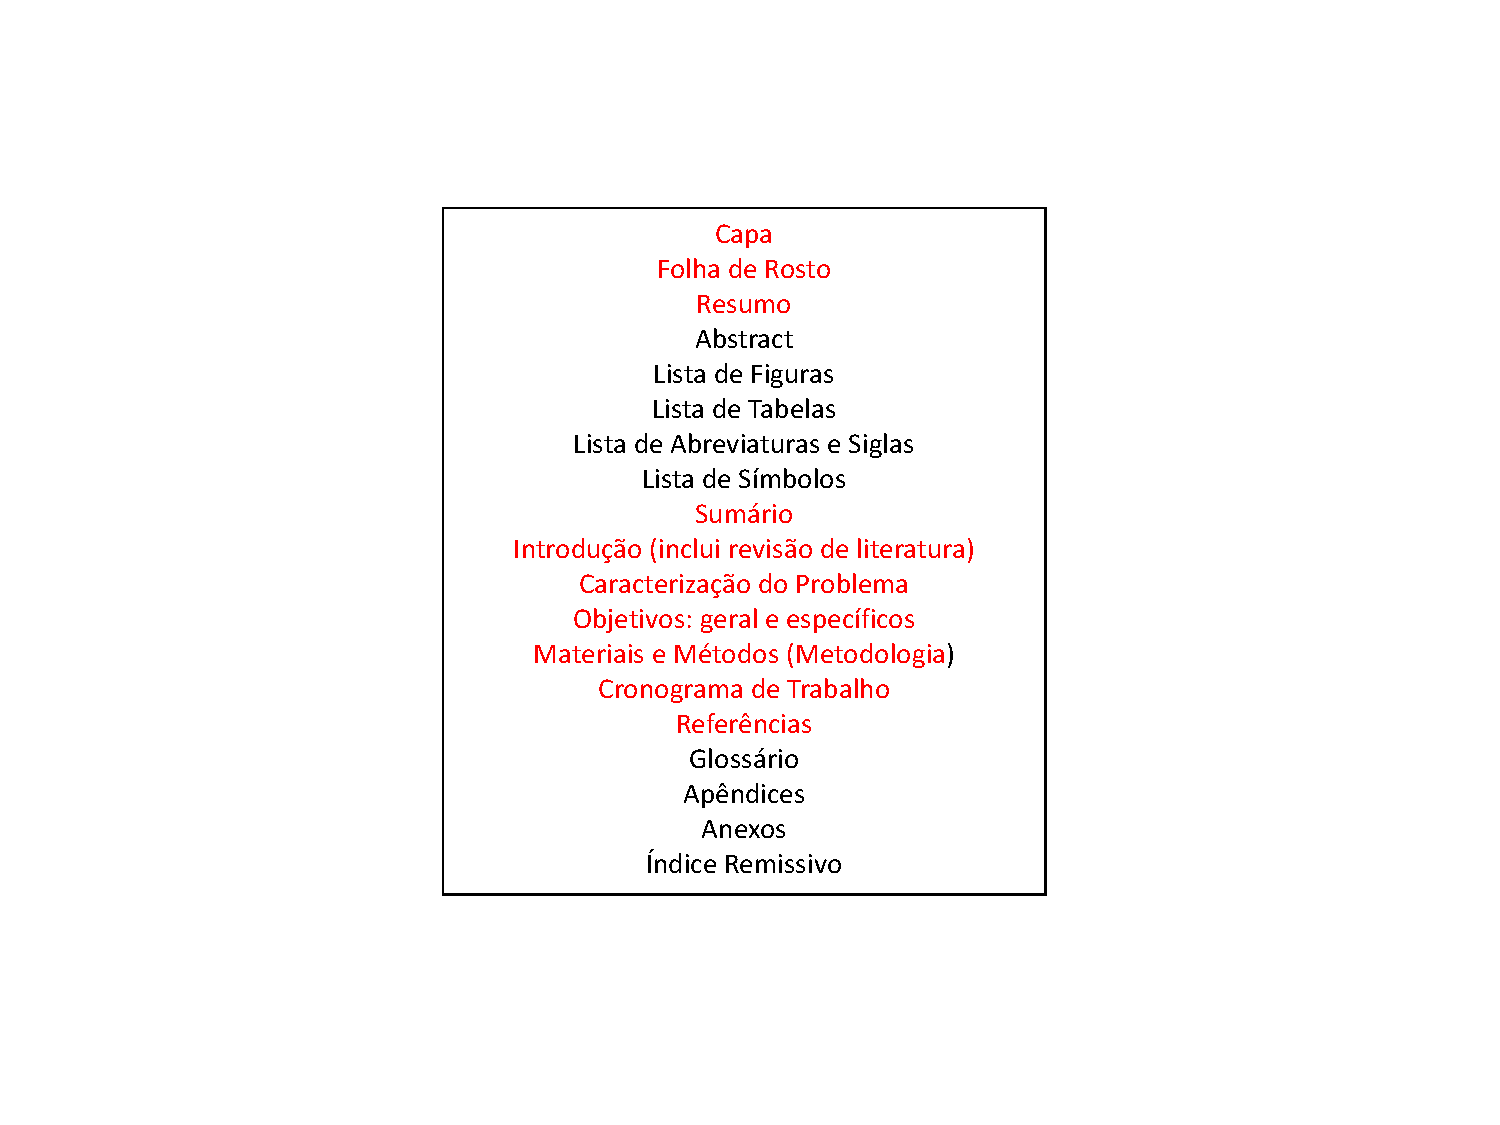
\includegraphics[width=0.6\textwidth]{./04-figuras/estrutura-projeto-pesquisa}
    \label{fig:estrutura-projeto-pesquisa}
\end{figure}

Você deverá editar o arquivo principal {\ttfamily meuTrabalhoAcademico.tex} para fazer os ajustes necessários, reiterando que as estruturas apresentadas são mera sugestão.

A inclusão de reticências (\ldots) no texto deverá ser feita através de um comando especial denominado \verb|\ldots| \cite{LaTeX2014}. Assim esse comando deverá ser utilizado ao invés da digitação de três pontos.

Para melhor entendimento do uso do estilo de formatação, aconselha-se que o potencial usuário analise os comandos existentes no arquivo {\ttfamily main.tex} e os resultados obtidos no arquivo {\ttfamily main.pdf} depois do processamento pelo software \LaTeX{} + \textsc{Bib}\TeX{} \cite{LaTeX2014,BibTeX2014}.
Recomenda-se a consulta ao material de referência do software para a sua correta utilização \cite{Lamport1986,Buerger1989,Kopka2003,Mittelbach2004}.

Finalmente, este modelo apresenta um arquivo {\ttfamily makefile} para agilizar a compilação do documento \LaTeX{} e do \textsc{Bib}\TeX{}. portanto, para gerar o documento final no formato PDF, basta apenas executar o comando {\ttfamily make all} no linux. Para limpar os arquivos temporários, basta digitar o comando {\ttfamily make clean}.

O estilo de documento utilizado é o {\ttfamily abntex2}.
Através desse estilo a constituição do documento torna-se facilitada, uma vez que o mesmo possui comandos especiais para auxiliar a distribuição/definição das diversas partes constituintes do projeto.
Esse estilo é baseado nas normas da ABNT\index{ABNT}.

Maiores detalhes relacionados aos comandos existentes no estilo poderão ser adquiridos através da documentação disponível no site \href{https://code.google.com/p/abntex2/}{https://code.google.com/p/abntex2/} \cite{abnTeX22014b}.

Uma das principais vantagens do uso do estilo de formatação para \LaTeX{}  é a formatação \textit{automática} dos elementos que compõem um documento acadêmico, tais como capa, folha de rosto, dedicatória, agradecimentos, epígrafe, resumo, abstract, listas de figuras, tabelas, siglas e símbolos, sumário, capítulos, referências, etc.

% -----------------------------------------------------------------------------
% Novo apêndice
% -----------------------------------------------------------------------------

\chapter{Sobre as ilustrações}
\label{chap:apSobreIlust}

A seguir ilustra-se a forma de incluir ilustrações no corpo do texto. Pela norma figuras, tabelas, quadros, equações, quadros, algoritmos, diagrama, etc. são tipos específicos de ilustrações. As ilustrações (pelo menos alguns tipos específicos) serão indexadas automática em suas respectivas listas.

A numeração sequencial de figuras, tabelas e equações ocorre de modo automático.

Referências cruzadas são obtidas através dos comandos \verb|\label{}| e \verb|\ref{}|. Por exemplo, não é necessário saber que o número de certo capítulo é \ref{chap:fundamentacaoTeorica} para colocar o seu número no texto. Alternativamente se pode usar desta forma: \autoref{chap:fundamentacaoTeorica}. Isto facilita muito a inserção, remoção ou relocação de elementos numerados no texto (fato corriqueiro na escrita e correção de um documento acadêmico) sem a necessidade de renumerá-los todos.

\section{Figuras}
\label{sec:figuras}

Abaixo é apresentado um exemplo de figura.

A \autoref{fig:kdtree} aparece automaticamente na lista de figuras.

Para uso avançado de imagens no \LaTeX{}, recomenda-se a consulta de literatura especializada \cite{Goossens2007}.

\begin{figure}[!htb]
    \centering
    \caption{Exemplo da estrutura de uma árvore KD}
    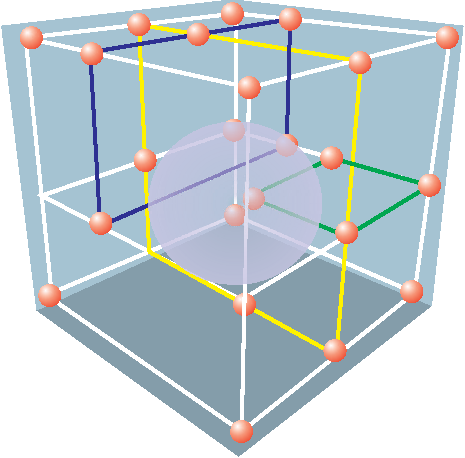
\includegraphics[width=0.5\textwidth]{./04-figuras/figura-exemplo}
    \fonte{\citeonline{Souza2012}}
    \label{fig:kdtree}
\end{figure}

\section{Quadros e tabelas}
\label{sec:tabelas}

Também é apresentado o exemplo do \autoref{qua:comparabd} e da \autoref{tab:testes}, que aparece automaticamente na lista de quadros e tabelas.

Informações sobre a construção de tabelas no \LaTeX{} podem ser encontradas na literatura especializada \cite{Lamport1986,Buerger1989,Kopka2003,Mittelbach2004}.

\begin{quadro}[!htb]
    \centering
    \caption{Hierarquia de restrições das questões.\label{qua:comparabd}}
    \begin{tabular}{|p{7cm}|p{7cm}|}
        \hline
        \textbf{BD Relacionais} & \textbf{BD Orientados a Objetos} \\
        \hline
        Os dados são passivos, ou seja, certas operações limitadas podem ser automaticamente acionadas quando os dados são usados. Os dados são ativos, ou seja, as solicitações fazem com que os objetos executem seus métodos. & Os processos que usam dados mudam constantemente. \\
        \hline
    \end{tabular}
    \fonte{\citeonline{Carvalho2001}}
\end{quadro}


Muitos confundem, mas existem diferenças entre tabelas e quadros.

Um quadro é formado por linhas horizontais e verticais, sendo, portanto ``fechado''. Você deverá utilizar um quadro quando o conteúdo é majoritariamente não-numérico. O número do quadro e o título vem acima do quadro, e a fonte, deve vir abaixo.

Uma tabela é formada apenas por linhas verticais, sendo, portanto ``aberta''. Você deverá utilizar uma tabela quando o conteúdo é majoritariamente numérico. O número da tabela e o título vem acima da tabela, e a fonte, deve vir abaixo, tal como no quadro.

Exemplo de tabela:

\begin{table}[!htb]
    \centering
    \caption[Resultado dos testes]{Resultado dos testes.
    \label{tab:testes}}
    \begin{tabular}{rrrrr}
        \toprule
            & Valores 1 & Valores 2 & Valores 3 & Valores 4 \\
        \midrule
            Caso 1 & 0,86 & 0,77 & 0,81 & 163 \\
            Caso 2 & 0,19 & 0,74 & 0,25 & 180 \\
            Caso 3 & 1,00 & 1,00 & 1,00 & 170 \\
        \bottomrule
    \end{tabular}
\end{table}


\section{Equações}
\label{sec:equacoes}

A transformada de Laplace é dada na \autoref{eq:laplace}, enquanto a Eq. \ref{eq:dft} apresenta a formulação da transformada discreta de Fourier bidimensional\footnote{Deve-se reparar na formatação esteticamente perfeita destas equações.}. Observe que utilizamos propositalmente duas formas distintas para referenciar as equações.

\begin{equation}
    X(s) = \int\limits_{t = -\infty}^{\infty} x(t) \, \text{e}^{-st} \, dt
    \label{eq:laplace}
\end{equation}

\begin{equation}
    F(u, v) = \sum_{m = 0}^{M - 1} \sum_{n = 0}^{N - 1} f(m, n) \exp \left[ -j 2 \pi \left( \frac{u m}{M} + \frac{v n}{N} \right) \right]
    \label{eq:dft}
\end{equation}

\section{Algoritmos}\label{sec:algoritmos}

Os algoritmos devem ser feitos segundo o modelo abaixo. Para isso, utilizar o pacote {\ttfamily algorithm2e} no início do arquivo principal como neste exemplo.
\\
\\

\begin{algorithm}
    \caption{Algoritmo para remoção aleatória de vértices}
    \KwIn{o número $n$ de vértices a remover, grafo original $G(V, E)$}
    \KwOut{grafo reduzido $G'(V,E)$}
    $removidos \leftarrow 0$ \\
    \While {removidos $<$ n } {
        $v \leftarrow$ Random$(1, ..., k) \in V$ \\
            \For {$u \in adjacentes(v)$} {
                remove aresta (u, v)\\
                $removidos \leftarrow removidos + 1$\\
            }
            \If {há  componentes desconectados} {
                remove os componentes desconectados\\
            }
        }
\end{algorithm}


% -----------------------------------------------------------------------------
% Novo apêndice
% -----------------------------------------------------------------------------

\chapter{Sobre as listas}
\label{chap:apSobreLista}

Para construir listas de "\textit{bullets}"{} ou listas enumeradas, inclusive listas aninhadas, é utilizado o pacote \verb|paralist|.

O exemplo a seguir ilustra duas listas não numeradas aninhadas, utilizando o ambiente \verb|\itemize|. Observe a indentação, bem como a mudança automática do tipo de "\textit{bullet}"{} nas listas aninhadas.

\begin{itemize}
    \item item não numerado 1
    \item item não numerado 2
    \begin{itemize}
        \item subitem não numerado 1
        \item subitem não numerado 2
        \item subitem não numerado 3
    \end{itemize}
    \item item não numerado 3
\end{itemize}

Por outro lado, o exemplo a seguir ilustra duas listas numeradas aninhadas, utilizando o ambiente \verb|\enumerate|. Observe a numeração progressiva e indentação das listas aninhadas.

\begin{enumerate}
    \item item numerado 1
    \item item numerado 2
    \begin{enumerate}
        \item subitem numerado 1
        \item subitem numerado 2
        \item subitem numerado 3
    \end{enumerate}
    \item item numerado 3
\end{enumerate}

Cabe ressaltar que os ambientes \verb|\itemize| e \verb|\enumerate| podem ser utilizados alternativamente. No entanto, durante a compilação pdflatex são apresentados erros associados a estes ambientes, porém o pdf é gerado corretamente. Trata-se de um "\textit{bug}"{} que ainda não conseguimos resolver. Caso conheça a solução, por favor, comunique-nos para que possamos incluí-la numa futura atualização deste modelo.

% -----------------------------------------------------------------------------
% Novo apêndice
% -----------------------------------------------------------------------------

\chapter{Sobre citações e chamadas de referências}
\label{chap:apSobreCita}

Citações são trechos transcritos ou informações retiradas das publicações consultadas para a realização do trabalho.
As citações são utilizadas no texto com o propósito de esclarecer, completar, embasar ou corroborar as ideias do autor.

Todas as publicações consultadas e efetivamente utilizadas (por meio de citações) devem ser listadas, obrigatoriamente, nas referências bibliográficas, de forma a preservar os direitos autorais e intelectuais.

A norma ABNT NBR:10520-2002 classifica as citações em: citações livres e citações literais.

\section{Citações livres}
\label{sec:citacoesLivres}

Nas citações livres, reproduzem-se as ideias e informações de um autor, sem, entretanto, ``copiar letra por letra'' o texto do autor. Sendo assim, não há muito a dizer sobre como fazer citações livres, exceto que há que se tomar o devido cuidado com o "recortar e colar e modificar"{} para que não se caracterize plágio.

Quanto à chamada da referência, ela pode ser feita de duas maneiras distintas, conforme o nome do(s) autor(es) façam parte do seu texto ou não. Os exemplos a seguir ilustram estas duas possibilidades.

Enquanto \citeonline{Maturana2003} defendem uma epistemologia baseada na biologia. Para os autores, é necessário rever \ldots.

Por outro lado, \citeonline{Barbosa2004} contra-argumenta afirmando que \ldots.

Acima, as chamadas de referências foram feitas com o comando \verb|\citeonline{chave}|, que produzirá a formatação correta, conforme a norma ABNT.

Observe que em ambos os casos anteriores, a frase fica incompleta e incompreensível caso as palavras "Maturana e Varela"{} e "Barbosa et al."{} não sejam "pronunciadas"{}. Ou seja, os nomes dos autores fazem parte da frase. Neste caso, a formatação automática da chamada de referência coloca os nomes dos autores seguido, entre parêntesis pelo ano de publicação da obra referenciada. Isso apenas no caso em que se usa o esquema autor-ano, que é \textit{padrão} neste modelo \LaTeX{}.

A segunda maneira de fazer uma chamada de referência deve ser utilizada quando se quer evitar uma interrupção na sequência do texto, o que poderia, eventualmente, prejudicar a leitura.

Assim, a citação livre é feita e imediatamente após a obra referenciada deve ser colocada entre parênteses. Porém, neste caso específico, o nome do autor deve vir em caixa alta, seguido do ano da publicação, como nos exemplos a seguir.

Há defensores da epistemologia baseada na biologia que argumentam em favor da necessidade de \ldots \cite{Maturana2003}.

Por outro lado, há os que contra-argumentam afirmando que \ldots  \cite{Barbosa2004}.

Nos dois casos imediatamente acima a chamada de referência deve ser feita com o comando \verb|\cite{chave}|, que produzirá a formatação correta, conforme a norma ABNT.

Observe que o estilo de redação das frases teve que ser modificado para torná-las compreensíveis sem a menção explícita dos nomes dos autores. Estes agora não são parte integrante da frase, ficam entre parêntesis. Neste caso, a formatação automática da chamada de referência coloca, entre parêntesis, os nomes dos autores seguido pelo ano de publicação da obra referenciada. Novamente, apenas no caso em que se usa o esquema autor-ano, que é \textit{padrão} neste modelo \LaTeX{}.

Por fim, cabe chamar a atenção para o detalhe do termo \textit{et al.} que deve ser utilizado quando o trabalho citado possui mais de três autores. Esse recurso é automatizado pelo estilo {\ttfamily abntex2}. Caso não haja desejo em abreviar o nome dos demais autores através do termo \textit{et al.}, deve-se incluir a opção {\ttfamily abnt-no-etal-label}.

\section{Citações literais}
\label{sec:citacoesLiterais}

Nas citações literais, reproduzem-se as ideias e informações de um autor, exatamente como este a expressou, ou seja, faz-se uma ``cópia letra por letra'' do texto do autor. Sendo assim, obviamente, a obra citada deve ser referenciada, sob pena de se caracterizar plágio.

Quanto à chamada da referência, ela pode ser feita de qualquer das duas maneiras mencionadas na \autoref{sec:citacoesLivres}, conforme o nome do(s) autor(es) façam parte do seu texto ou não.

Há duas maneiras distintas de se fazer uma citação literal, conforme o trecho citado seja longo ou curto.

Quando o trecho citado é longo (4 ou mais linhas) deve-se usar um parágrafo específico para a citação, na forma de um texto recuado (4 cm da margem esquerda), com tamanho de letra menor do aquela utilizada no texto e espaçamento entrelinhas simples. Veja o exemplo abaixo.

\begin{citacao}
    Desse modo, opera-se uma ruptura decisiva entre a reflexividade filosófica, isto é a possibilidade do sujeito de pensar e de refletir, e a objetividade científica.     Encontramo-nos num ponto em que o conhecimento científico está sem consciência. Sem consciência moral, sem consciência reflexiva e também subjetiva. Cada vez mais o desenvolvimento extraordinário do conhecimento científico vai tornar menos praticável a própria possibilidade de reflexão do sujeito sobre a sua pesquisa \cite[p.~28]{Silva2000}.
\end{citacao}

Para se criar o efeito demonstrado na citação anterior, deve-se utilizar o comando:

\begin{verbatim}
\begin{citacao}
<citacao>
\end{citacao}
\end{verbatim}

Acima, para a chamada da referência o comando \verb|\cite[p.~28]{Silva2000}| foi utilizado, visto que os nomes dos autores não são parte do trecho citado.

Observe ainda que foi indicado o número da página da obra citada que contém o trecho citado. A localização precisa do trecho citado deve ser indicada sempre, exceto para artigos científicos (tipicamente com poucas páginas, o que geralmente não é o caso de artigos de revisão de literatura) e outros documentos com "poucas"{} páginas.

Alternativamente, é possível construir uma frase que contenha os autores, e irá encaminhar (por assim dizer) a citação literal. Assim sendo, note que pode após a citação literal não mais aparece o nome dos autores, visto que já se encontra no texto. Veja o exemplo seguinte.

No entanto, \citeonline[p.~33]{Silva2000}, ao fazerem as suas críticas à ciência moderna, afirmam:

\begin{citacao}
    Mas o curioso é que o conhecimento científico que descobriu os meios realmente extraordinários para, por exemplo, ver aquilo que se passa no nosso sol, para tentar conceber a estrutura das estrelas extremamente distantes, e até mesmo para tentar pesar o universo, o que é algo de extrema utilidade, o conhecimento científico que multiplicou seus meios de observação e de concepção do universo, dos objetos, está completamente cego, se quiser considerar-se apenas a si próprio!
\end{citacao}

Já quando o trecho citado é curto (3 ou menos linhas) ele deve inserido diretamente no texto entre aspas. Veja os dois exemplos seguintes, cada qual utilizando uma forma de chamada de referência.

A epistemologia baseada na biologia parte do princípio de que ``assumo que não posso fazer referência a entidades independentes de mim para construir meu explicar'' \cite[p.~35]{Maturana2003}.

A epistemologia baseada na biologia de \citeonline[p.~35]{Maturana2003} parte do princípio de que ``assumo que não posso fazer referência a entidades independentes de mim para construir meu explicar''.

Finalmente, e isto vale para citações curtas ou longas, caso seja necessário inserir ou suprimir (modificar de modo geral) qualquer palavra ou frase no trecho citado literalmente, qualquer que seja a finalidade, isto deve ser feito colocando sua intervenção entre colchetes retos e deve ser indicado explicitamente ao final da citação. Veja o exemplo seguinte.

A epistemologia baseada na biologia parte do princípio de que ``assumo que não posso fazer referencia [\textit{sic}] a \underline{entidades independentes} de mim [realidade objetiva] para construir meu explicar'' \cite[p.~35, comentários e grifo nosso]{Maturana2003}.

\section{Mais detalhes sobre as chamadas de referências}
\label{sec:referUtilizadas}

A seguir há mais exemplos dos comandos para as chamadas de referências e o resultado produzido.

\citeonline{Maturana2003} \ \ \  \verb|\citeonline{Maturana2003}|\\
\citeonline{Barbosa2004} \ \ \   \verb|\citeonline{Barbosa2004}|\\
\cite[p.~28]{Silva2000} \ \ \  \verb|\cite[p.~28]{Silva2000}|\\
\citeonline[p.~33]{Silva2000} \ \ \   \verb|\citeonline[p.~33]{v}|\\
\cite[p.~35]{Maturana2003} \ \ \   \verb|\cite[p.~35]{Maturana2003}|\\
\citeonline[p.~35]{Maturana2003} \ \ \   \verb|\citeonline[p.~35]{Maturana2003}|\\
\cite{Barbosa2004,Maturana2003} \ \ \   \verb|\cite{Barbosa2004,Maturana2003}|\\

Há que se tomar bastante cuidado com referências cujos autores têm nomes compostos, tipo João de Souza Júnior ou Antônio José da Silva Filho. Para que a formatação seja correta, os nomes dos autores no arquivo {\ttfamily .bib} deverá ser cadastrado de uma forma específica. Para maiores detalhes, veja o \autopageref{chap:anexoB} \footnote{O texto do anexo é de inteira responsabilidade do autor devidamente referenciado.}.

Os exemplos abaixo ilustram a formatação correta.

\cite[p.~28]{vanGELDER1998} \ \ \ \ \  \verb|\cite[p.~28]{vanGELDER1998}|\\
\citeonline[p.~28]{vanGELDER1998} \ \ \ \ \  \verb|\citeonline[p.~28]{vanGELDER1998}|\\

Observe que, a despeito do que está dito no \autoref{chap:anexoB}, ainda há falhas na formatação ABNT de nomes tipo \verb|van Gelder| quando utilizados em chamadas de referências que fazem parte do texto (\textit{e.g.}, \verb|\citeonline{vanGELDER1998}| que deveria produzir \verb|van Gelder (1998)|). Este problema pode ser contornado facilmente, simplesmente evitando o uso dessa forma de chamada de referência, preferindo sempre nestes casos, o uso da forma \textit{e.g.}, \verb|\cite{vanGELDER1998}| que será formatada corretamente, produzindo \verb|(van GELDER, 1998)|.

Observe ainda o caso em que é feita duas citações juntas \cite{Santos2003, Neubert2001} e como citar endereços Web \cite{IRL2014}.

% -----------------------------------------------------------------------------
% Novo apêndice
% -----------------------------------------------------------------------------

\chapter{Sobre as referências bibliográficas}
\label{chap:apSobreRefer}

A bibliografia é feita no padrão \textsc{Bib}\TeX{}. As referências são colocadas em um arquivo separado. Os elementos de cada item bibliográfico que devem constar nas referências bibliográficas são apresentados a seguir. Tais referências bibliográficas devem seguir a norma \citeonline{NBR6023:2002} da ABNT\footnote{As normas técnicas da ABNT não são gratuitas.}.

\section{Entradas de referências}
\label{sec:entradasRefs}

Entradas são objetos de citação bibliográficas. Dito de outra forma, são as categorias dos tipos de documentos e materiais componentes da bibliografia. A classe abn\TeX{} define as seguintes entradas:

\begin{verbatim}
@book
@inbook
@article
@phdthesis
@mastersthesis
@monography
@techreport
@manual
@proceedings
@inproceedings
@journalpart
@booklet
@patent
@unpublished
@misc
\end{verbatim}

Cada entrada é formatada pelo pacote \citeonline{abnTeX22014d} de uma forma específica. Algumas entradas foram introduzidas especificamente para atender à norma \citeonline{NBR6023:2002}, são elas: \verb|@monography|, \verb|@journalpart|,\verb|@patent|. As demais entradas são padrão \textsc{Bib}\TeX{}. Para maiores detalhes, refira-se a \citeonline{abnTeX22014d}, \citeonline{abnTeX22014b}, \citeonline{abnTeX22014c}.

A entrada \verb|@monography| é utilizada para cadastrar referências a trabalhos de conclusão de curso, monografias de cursos de especialização (pós-graduação \textit{lato sensu}), e outros trabalhos monográficos, exceto dissertação de mestrado e tese de doutorado. Eu particularmente, não considero que a formatação deste tipo de entrada está adequado. Para um trabalho de conclusão de curso (TCC) de curso de graduação, que deveria ser formatado como "[\ldots] Trabalho de Conclusão de Curso (Bacharelado em Engenharia de Computação) [\ldots]"{}; no entanto o uso de \verb|@monography| irá produzir "[\ldots] Monografia (Bacharelado em Engenharia de Computação) [\ldots]"{}. A própria  \citeonline{NBR6023:2002}, na seção 8.11.4, apresenta um exemplo com a formatação diferente daquela proporcionada por \citeonline{abnTeX22014d}.

A entrada \verb|@journalpart| é utilizada, conforme diz o manual \cite{abnTeX22014d}, para cadastrar referências e formatar partes de periódicos. Não fica claro o que se quer dizer com partes de journal. Em alguns casos, tais partes são artigos - e portanto, deveriam ser registradas como \verb|@article| - noutros casos, parece serem matérias ou textos em revistas ou jornais (não científicos). Salvo melhor juízo, me parece que esta entrada deve ser utilizada apenas neste último contexto.

A entrada \verb|@patent| é utilizada, obviamente, para cadastrar referências a patentes.

Todavia, o fato é que a normalização de referências conforme a norma \citeonline{NBR6023:2002} requer que muitos dos campos do \textsc{Bib}\TeX{} sejam adaptados. Sendo mais explícito, ao baixar um arquivo {\ttfamily .bib} de um trabalho, principalmente ser for internacional, e inserí-lo "\textit{as is}"{} em suas referências, há grande chance dessa referência ser formatada de modo errado, no que concerne à norma \citeonline{NBR6023:2002}. Isso é especialmente válido em alguns tipos de documentos de largo uso no meio acadêmico afim às áreas de Ciências Exatas, da Terra e Engenharias.

Diante disso, para evitar erros de formatação, o correto é após baixar o arquivo {\ttfamily .bib} de um trabalho, editá-lo com um editor ASCII (usando codificação UTF8), para verificar se os campos descritores que o \textit{publishers} original utilizou são aqueles requeridos pela norma ABNT.

Neste contexto, e para esta finalidade, nas seções seguintes é apresentado uma série de exemplos, quase todos, utilizados como exemplos na própria norma \citeonline{NBR6023:2002}. Para detalhes dos campos utilizados confira o arquivo {\ttfamily myRefs.bib}. Deve-se estar atento para o fato de que o uso de um sistema de gerenciamento de referências para abrir e/ou editar o arquivo {\ttfamily myRefs.bib}, pode ocultar campos utilizados pela norma ABNT e, por outro lado, exibir campos não utilizados por ela. Ou seja, o aplicativo deve ser configurado adequadamente para exibir \textbf{todos os campos}, mesmo os opcionais.

\section{Notas de rodapé}
\label{sec:notasRodape}

A norma \citeonline{NBR10520:2002}, em sua seção \textbf{7 Notas de rodapé}, classifica as notas de rodapé em duas categorias: notas explicativas\footnote{é o tipo mais comum de notas que destacam, explicam e/ou complementam o que foi dito no corpo do texto, como esta nota de rodapé, por exemplo.} e notas de referências. Já as notas de referências, como o próprio nome ja indica, são utilizadas para colocar referências e/ou chamadas de referências sob certas condições.

\subsection{Notas de referências: uso de idem, ibidem, opus citatus e outros}
\label{subsec:notasRefs}

Como indica o próprio nome, as notas de referências se prestam como recurso auxiliar para referenciação de bibliografia, e seu uso e aplicação são descritos na seção \textbf{7.1 Notas de referência} da norma \citeonline{NBR10520:2002}.

Estes recursos se referem ao uso de certas expressões consagradas para facilitar a elaboração de referencias. São eles:

\begin{itemize}
    \item idem = mesmo autor,
    \item ibidem = mesma obra,
    \item opus citatum = obra citada,
    \item locus citatum = no lugar citado,
    \item passim = aqui e alí,
    \item cf = confira,
    \item et sequentia = e sequência.
\end{itemize}

Observe que estes recursos não se adequam para serem utilizados em listas de referências bibliográficas, nem tampouco no corpo do texto. Assim, devem ser utilizados apenas nas notas de referência posicionadas no rodapé \cite[p.~6]{abnTeX22014c}, quando se referem a uma referência já feita anteriormente no corpo do texto. Ademais, essas expressões fazem sentido apenas quando aplicadas a citações de uma única referência por vez. Enfim, trata-se mais de um recurso estilístico do que algo de primeira necessidade, pelo menos para o tipo de documento usualmente elaborados nas área de Ciências Exatas, da Terra e Engenharias.

Veja o uso desses tipos de expressões nos exemplos seguintes:

\Idem[p.~21]{abnTeX22014d}

\Ibidem[p.~7]{abnTeX22014c}

\opcit[p.~9]{abnTeX22014c}

\passim{abnTeX22014c}

\cfcite[p.~3]{abnTeX22014b}

\etseq[p.~6]{abnTeX22014c}

\section{Datas em referências}
\label{sec:datasBib}

Quando as chamadas de referências são feitas no modelo autor-ano, como é o caso deste modelo \LaTeX{}, é evidente que o autor e sobretudo o ano adquirem papel de destaque. No caso da data de publicação, esta deve sempre estar presente (é elemento essencial) e indicada em algarismos arábicos.

A norma ABNT não permite o uso de expressões do tipo "sem data"{} ("[s.d]") para indicar que não se sabe a data de publicação de certa referência bibliográfica. Assim sendo, quando a data não puder ser indicada precisamente, deve-se registrar uma data aproximada entre colchetes, conforme descrito a seguir:

[1971 ou 1972] \ \ \ \ \ um ano ou outro,

[1969?] \ \ \ \ \ ano provável,

[1973] \ \ \ \ \ ano certo, não indicada no item,

[entre 1906 e 1912] \ \ \ \ \ use intervalos menores de 20 anos,

[ca. 1960] \ \ \ \ \ \textit{circa} de ... ( data aproximada),

[197-] \ \ \ \ \ década certa,

[197-?] \ \ \ \ \ década provável,

[18--] \ \ \ \ \ século certo,

[18--?] \ \ \ \ \ século provável.

\end{apendicesenv}
          % Apêndices
% -----------------------------------------------------------------------------
% Anexos
% -----------------------------------------------------------------------------

\begin{anexosenv}
\partanexos

% -----------------------------------------------------------------------------
% Anexo A: Estrutura de entrevista com designer
% -----------------------------------------------------------------------------

\chapter{Estrutura de entrevista com designer}
\label{chap:anexoA}

\begin{itemize}
  \item Conte um pouco sobre seu \textit{background} na empresa.
  \item Contextualize, brevemente, a maneira como os processos de design são adotados na empresa, atualmente.
  \item Quais as maiores dificuldades e frustrações que você encontra no seu trabalho, como consequência dos processos atuais de design?
  \item Como são tomadas decisões de design na empresa? E no seu time? Quem são as pessoas envolvidas?
  \item Como você classifica a velocidade de desenvolvimento de novas interfaces de usuários atualmente? Por que?
  \item Você acredita que um \textit{design system} poderia ser uma opção plausível para alavancar a capacidade de escalabilidade do produto da empresa?
  \item Mais alguma idéia, dúvida ou comentário a respeito de \textit{design systems}?
\end{itemize}

% -----------------------------------------------------------------------------
% Anexo B: Estrutura de entrevista com desenvolvedor
% -----------------------------------------------------------------------------

\chapter{Estrutura de entrevista com desenvolvedor}
\label{chap:anexoB}

\begin{itemize}
  \item Conte um pouco sobre seu \textit{background} na empresa.
  \item Contextualize, brevemente, a maneira como os processos de desenvolvimento \textit{frontend} são adotados na empresa, atualmente.
  \item Quais as maiores dificuldades e frustrações que você encontra na plataforma durante o desenvolvimento de suas atividades?
  \item Você participa das decisões de design das suas entregas? Faz(ria) sentido para você participar? Por que?
  \item Como você classifica a velocidade de desenvolvimento de novas interfaces de usuários atualmente? Por que?
  \item Como você classifica o esforço para se realizar manutenção em interfaces de usuário já existentes na plataforma atualmente?
  \item De modo geral, como você classifica a atual arquitetura \textit{frontend} da plataforma a nível de escalabilidade e reusabilidade?
  \item Você já ouviu falar no termo \textit{design system}? Se sim, acredita que poderia ser uma abordagem plausível para impulsinar a capacidade de escalabilidade do produto da empresa?
  \item Mais alguma idéia, dúvida ou comentário a respeito de \textit{design systems}?
\end{itemize}

% -----------------------------------------------------------------------------
% Anexo C: Pesquisa de satisfação da arquitetura do produto da Dito
% -----------------------------------------------------------------------------

\chapter{Pesquisa de satisfação da arquitetura do produto da Dito}
\label{chap:anexoC}

\begin{itemize}
	\item Em uma escala de 1 a 10, sendo 1 extremamente lenta e 10 extremamente rápida, como você classificaria a velocidade de desenvolvimento de novas interfaces de usuário na plataforma da Dito?
	\item Em uma escala de 1 a 10, sendo 1 terrível e 10 excelente, como você classificaria o poder de reusabilidade de componentes na plataforma da Dito?
	\item Em uma escala de 1 a 10, sendo 1 terrível e 10 excelente, como você classificaria a capacidade de escalabilidade da plataforma da Dito?
\end{itemize}

\end{anexosenv}
             % Anexos
% -----------------------------------------------------------------------------
% Índice Remissivo
% -----------------------------------------------------------------------------

% -----------------------------------------------------------------------------
% Este comando gera automaticamente o índice remissivo para os termos definidos
% no corpo do documento.
% -----------------------------------------------------------------------------

\printindex

% -----------------------------------------------------------------------------
% Não é necessário editar este arquivo.
% -----------------------------------------------------------------------------
   % Índice Remissivo

\end{document}
